%\documentclass[9pt]{book}
\documentclass[landscape,14pt]{oblivoir}
    \usepackage{a4wide}
    \usepackage{palatino}
    \usepackage{newcent}
    \usepackage{amsmath,amsfonts,amssymb}
	\usepackage{graphics} % for pdf, bitmapped graphics files
	\usepackage{epsfig} % for postscript graphics files
	\usepackage{xcolor}
    \usepackage{hyperref}
    \usepackage{cancel}

\hypersetup{
    colorlinks=true,
    linkcolor=blue,
    filecolor=magenta,      
    urlcolor=cyan,
    pdftitle={Overleaf Example},
    pdfpagemode=FullScreen,
    }
    \urlstyle{same}
\usepackage{cuted}

    \setlength{\parindent}{0mm}
    \setlength{\textheight}{183.0mm}
    \setlength{\oddsidemargin}{-11.0mm}
    \setlength{\textwidth}{243.5mm}
   \setlength{\topmargin}{-30.0mm} 

\begin{document}

    \baselineskip 20pt
    \thispagestyle{empty}
    %!TEX root = ../main.tex
\setcounter{chapter}{7}
\setcounter{section}{0}
\section{Digitization}
\vspace{-8pt} \hrule \hrule \hrule \hrule \hrule  \vspace{12pt}
\begin{enumerate}
 \item Most control systems use digital computers (usually microprocessors) to implement the controller. 
 \item Sampler and A/D Converter, D/A Converter and ZOH (Zeroth-Order Holding), and Clock
 \item The computation of error signal $e(t)$ and the dynamic compensation $D_c(s)$ can all be accomplished in a digital computer. 
 \item Difference equation for discrete-time system $\leftrightarrow$ Differential equation for continuous-time system 
 \item Two basic techniques for finding the difference equations for the digital controller, from $D_c(s)$ to $D_d(z)$ 
 \begin{itemize}
  \item Discrete equivalent - section 8.3 
  \item Discrete design  - section 8.7 
 \end{itemize} 
 \item The analog output of the sensor is sampled and converted to a digital number in the analog-to-digital (A/D) converter. (Sampler and ADC)
 \begin{itemize}
  \item Conversion from the continuous analog signal $y(t)$ to the discrete digital samples $y(kT)$ occurs repeatedly at instants of time $T$ apart where $T$ is the sample period [$s$] and $1/T$ is the sample rate [$Hz$].
  \begin{align*}
   y(t) ~~~~ \rightarrow~~~~~y (k) = y(kT) ~~~~\mbox{with} ~~ t = kT  
  \end{align*}
  where $k$ is an integer and $T$ is a fixed value (sample period, or sampling time). 
  \item The sampled signal is $y(kT)$, where $k$ can take on any integer value. 
  \item It is often written simply as $y(k)$. We call this type of variable a discrete signal. 
 \end{itemize}  

\end{enumerate}

   
    \newpage
    %!TEX root = ../main.tex
\setcounter{chapter}{7}
\setcounter{section}{0}

%
\section{Digitization}
\vspace{-8pt} \hrule \hrule \hrule \hrule \hrule  \vspace{12pt}


\begin{enumerate}\addtocounter{enumi}{6}
 \item The D/A converter changes the digital binary number to an analog voltage, and a zeroth-order hold maintains the same voltage throughout the sample period $T$. (DAC and ZOH)

 \begin{itemize}
  \item Because each value of $u(kT)$ in Fig. 8.1(b) is held constant until the next value is available from the computer, the continuous value of $u(t)$ consists of steps (see Fig. 8.2) that, on average, are delayed from a fit to $u(kT)$ by $T/2$ as shown in the figure. 
  \item Sample rates should be at least 20 times the bandwidth in order to assure that the digital controller will match the performance of the continuous controller.
  \item If we simply incorporate this $T/2$ delay into a continuous analysis of the system, an excellent prediction results in, especially, for sample rates much slower than 20 times bandwidth.
 \end{itemize}
 \item A system having both discrete and continuous signals is called a `sampled data system'. 

\end{enumerate}

   
    \newpage
    %!TEX root = ../main.tex
\setcounter{chapter}{7}
\setcounter{section}{0}
\section{Digitization}
\vspace{-8pt} \hrule \hrule \hrule \hrule \hrule  \vspace{12pt}
\begin{figure}[!hb]
    \centering
    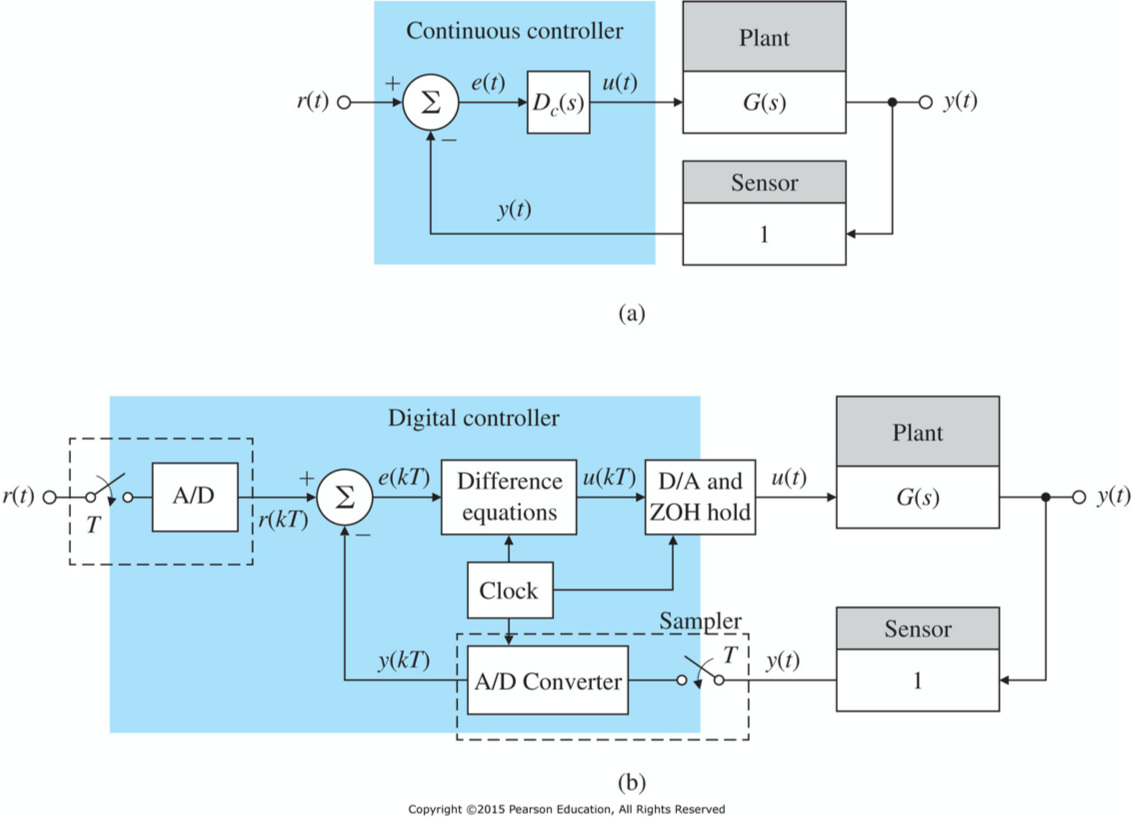
\includegraphics[width=20cm]{./FIG_Franklin/fig8-1.png}
\end{figure}   
    \newpage
    %!TEX root = ../main.tex
\setcounter{chapter}{7}
\setcounter{section}{0}
\section{Digitization}
\vspace{-8pt} \hrule \hrule \hrule \hrule \hrule  \vspace{12pt}
 \begin{itemize}
  \item Continuous-time signal: Both domain and range are continuous, $y(t)$

  \item Discrete-time signal: Domain is discrete and range is continuous, $y(k)$ or $y(kT)$

  \item Digital signal: Both domain and range are discrete, $y_d(k)$
    \begin{figure}[!hb]
        \centering
        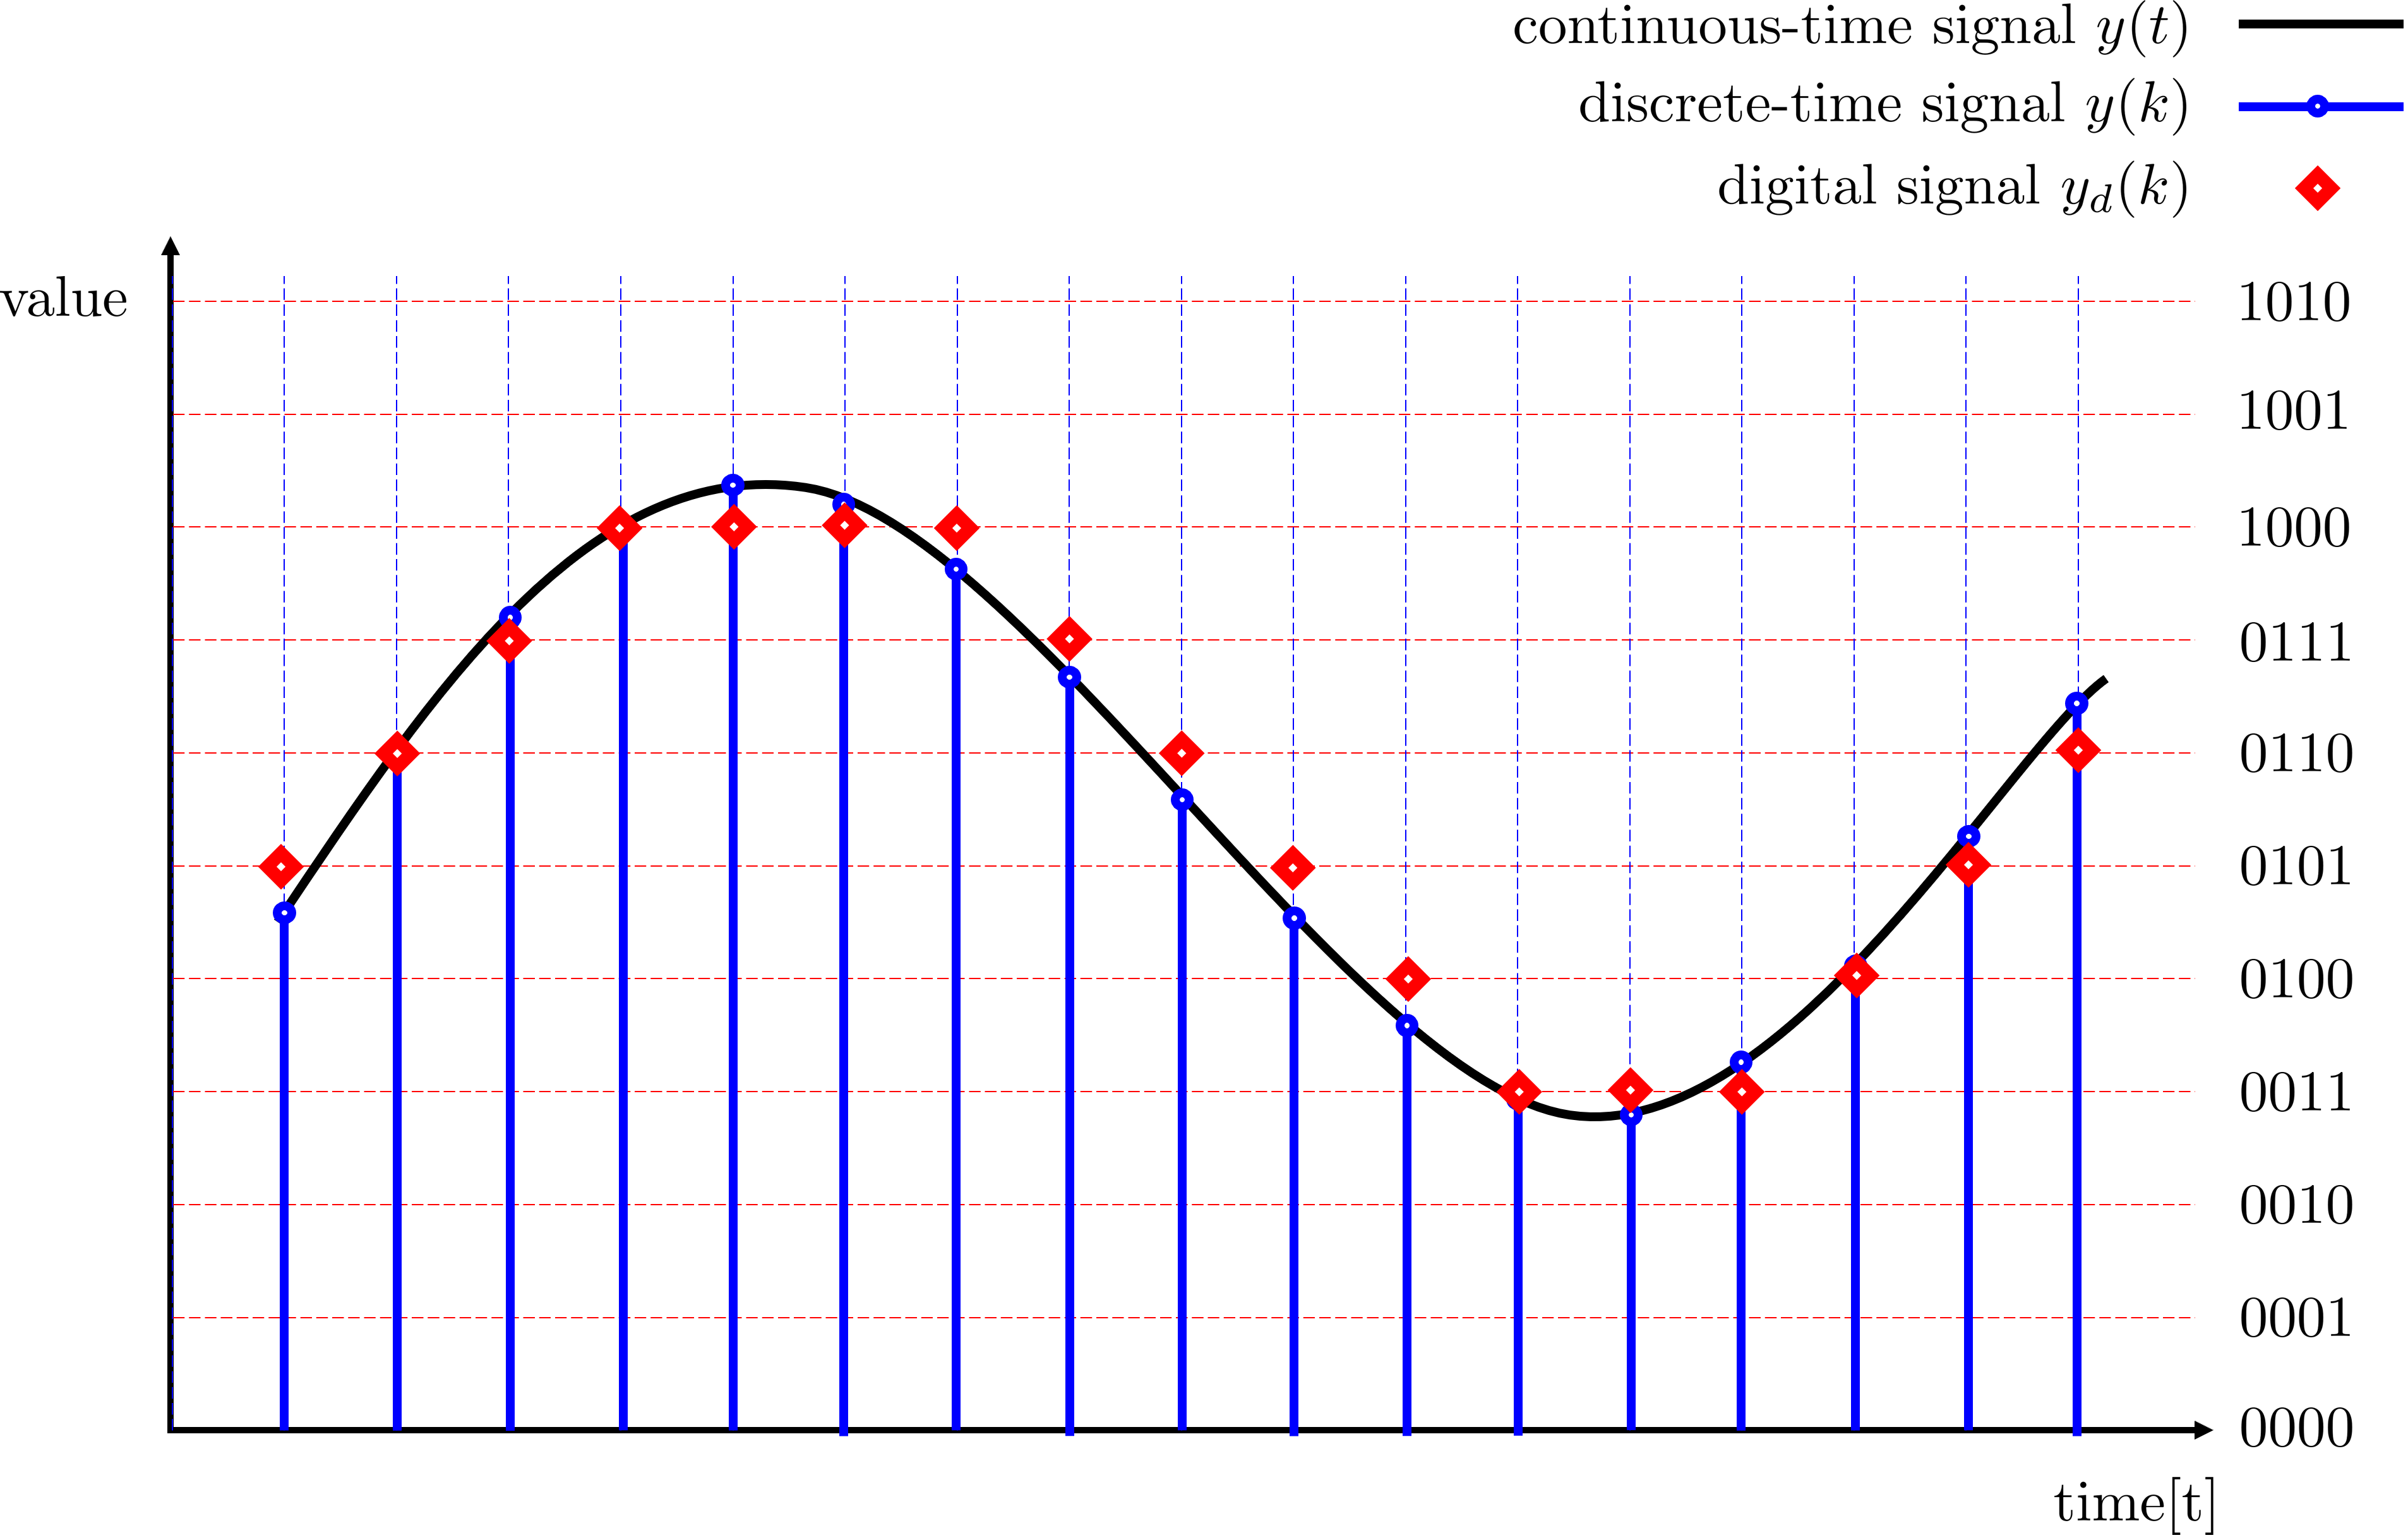
\includegraphics[width=20cm]{./FIG_Franklin/fig8-smc1.png}
    \end{figure}
 \end{itemize}    
    \newpage
    %!TEX root = ../main.tex
\setcounter{chapter}{7}
\setcounter{section}{0}
\section{Digitization}
\vspace{-8pt} \hrule \hrule \hrule \hrule \hrule  \vspace{12pt}

$\bigstar$ Dirac delta function is mathematically defined as:
\begin{enumerate}
	\item Approximation
	\begin{align*}
		F_{\Delta t}(t) = \begin{cases}1/\Delta t & 0 < t \leq \Delta t \\0 & otherwise \end{cases}\\
		\delta(t) =  \lim_{\Delta t\rightarrow 0} F_{\Delta t}(t) 
	\end{align*}
	    \begin{figure}[!h]
	        \centering
	        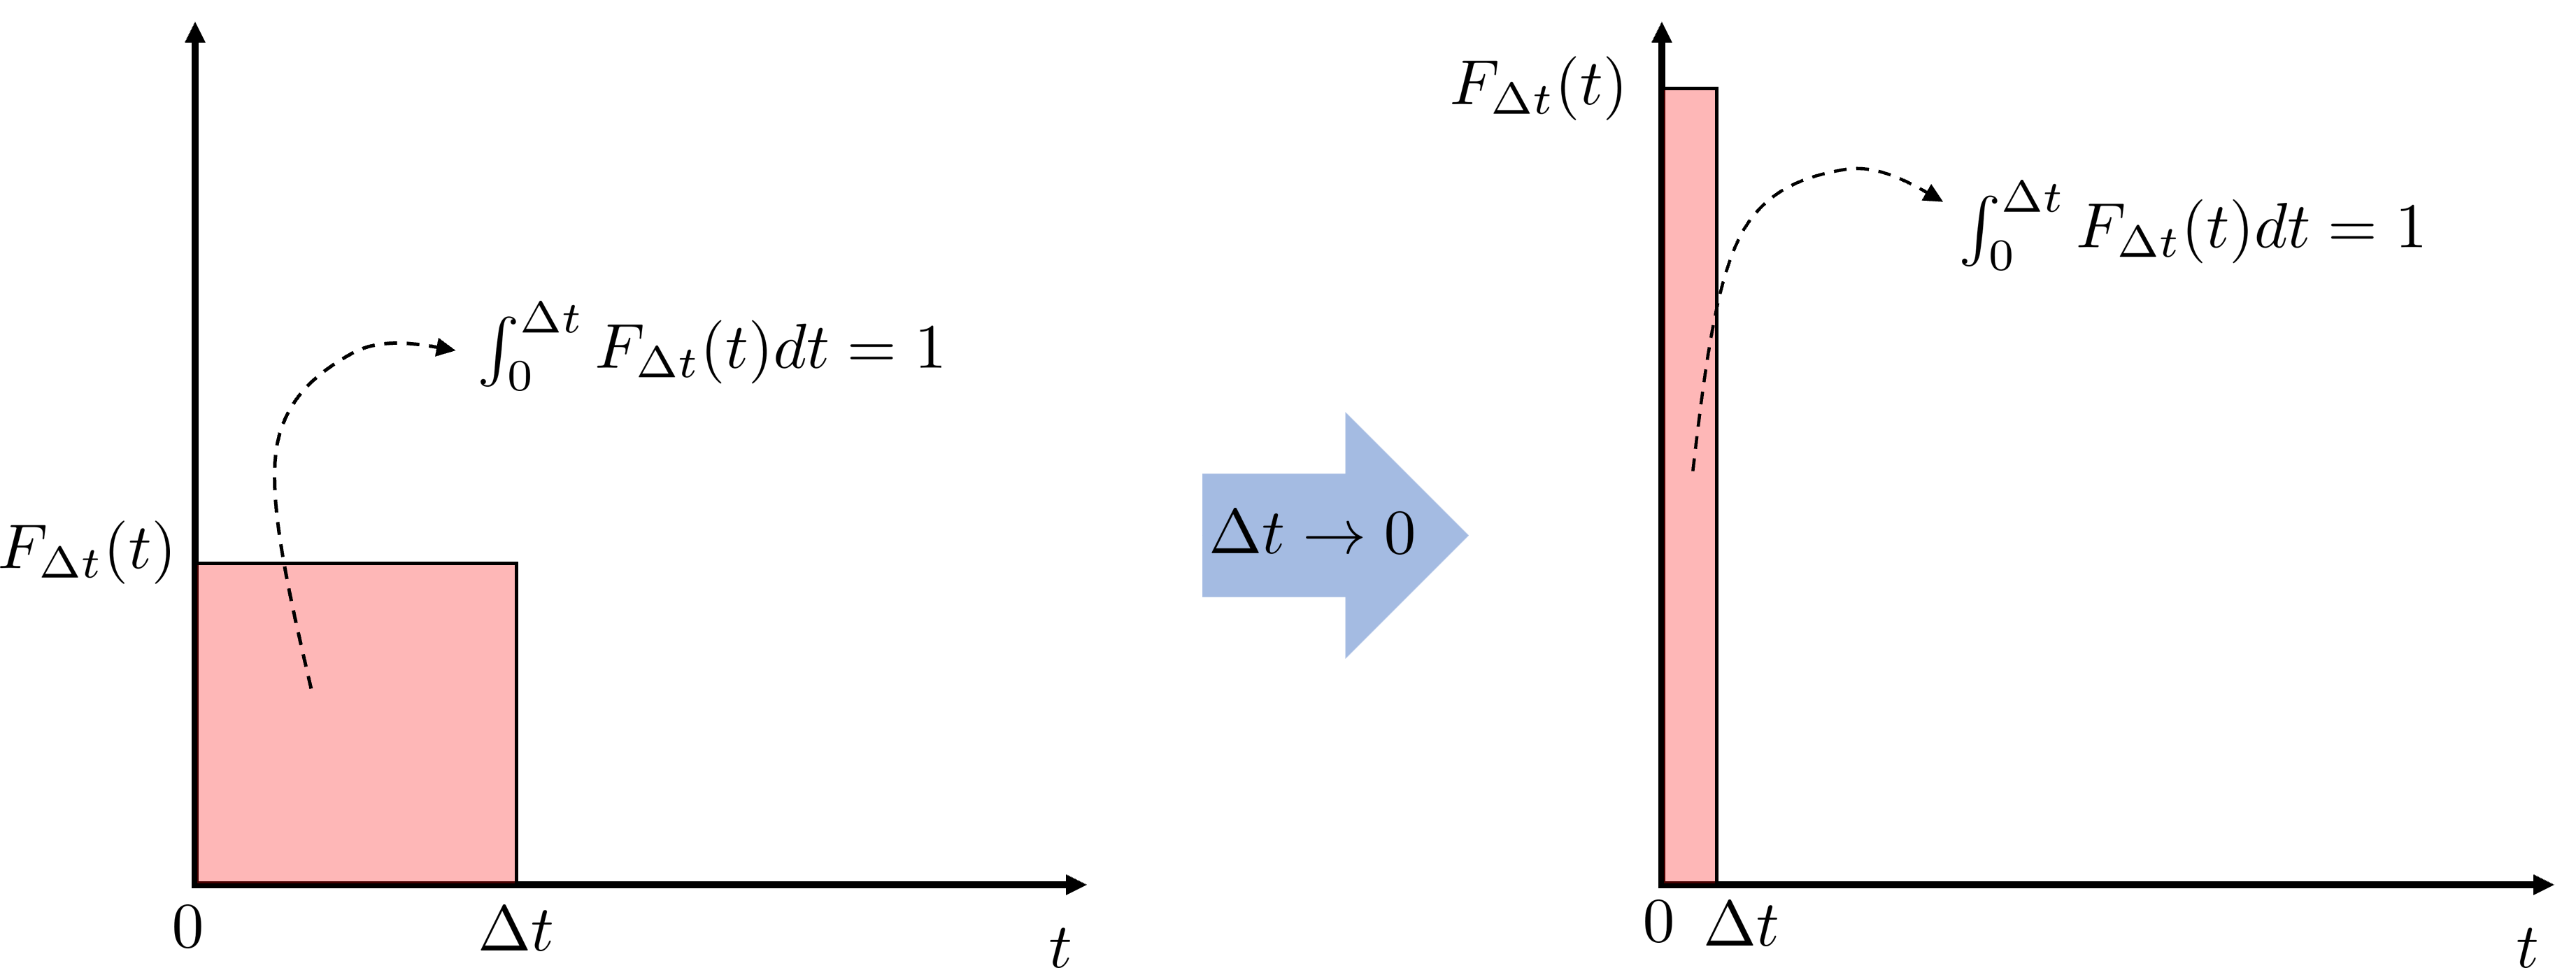
\includegraphics[width=20cm]{./FIG_Franklin/fig8-smc2.png}
	    \end{figure}

\end{enumerate}

   
    \newpage
    %!TEX root = ../main.tex
\setcounter{chapter}{7}
\setcounter{section}{0}
\section{Digitization}
\vspace{-8pt} \hrule \hrule \hrule \hrule \hrule  \vspace{12pt}

$\bigstar$ Unit step function
\begin{align*}
	1_k(t) = \frac{1}{1+e^{-2kt}}&&&& 1(t) = \begin{cases}1 & t \geq 0 \\0 & t< 0\end{cases}\\
	1(t) = \lim_{k \rightarrow \infty} 1_k(t) 
\end{align*}


	    \begin{figure}[!h]
	        \centering
	        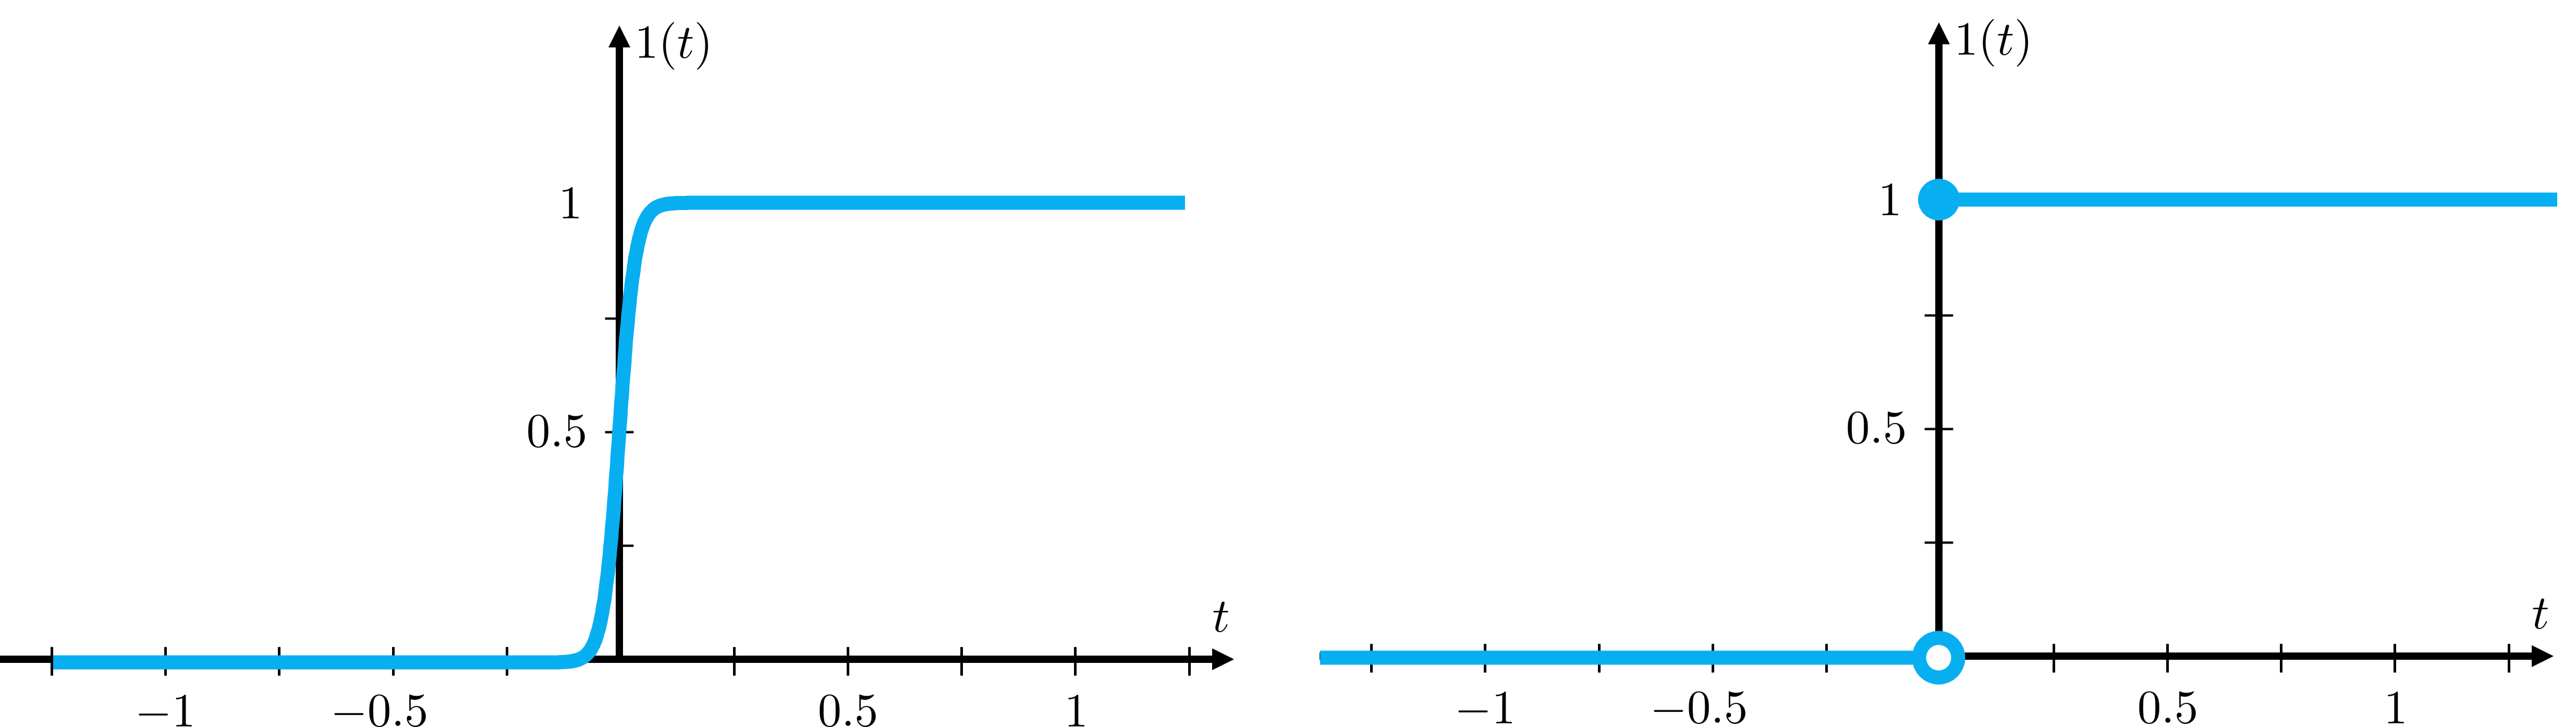
\includegraphics[width=18cm]{./FIG_Franklin/fig8-smc2_2.png}
	    \end{figure}


$\bigstar$ Useful Properties
 \begin{enumerate}
 	\item $\frac{d1(t)}{dt} = \delta(t) $ (수학적으로는 틀림, 개념적으로 사용)
 	\item $x(t)\delta(t-kT) = x(kT)\delta(t-kT)$
 	\item $\int_{-\infty}^{\infty} x(t) \delta(t-kT) dt= x(kT)$\\
		$ \because \int_{-\infty}^{\infty} x(t) \delta(t-kT)dt =\int_{-\infty}^{\infty} x(kT) \delta(t-kT) dt=x(kT)\int_{-\infty}^{\infty} \delta(t-kT) dt=x(kT)$
 	
 
 \end{enumerate}


   
    \newpage
    %!TEX root = ../main.tex
\setcounter{chapter}{7}
\setcounter{section}{0}
\section{Digitization}
\vspace{-8pt} \hrule \hrule \hrule \hrule \hrule  \vspace{12pt}

$\bigstar$ Sampling Process
	    \begin{figure}[!h]
	        \centering
	        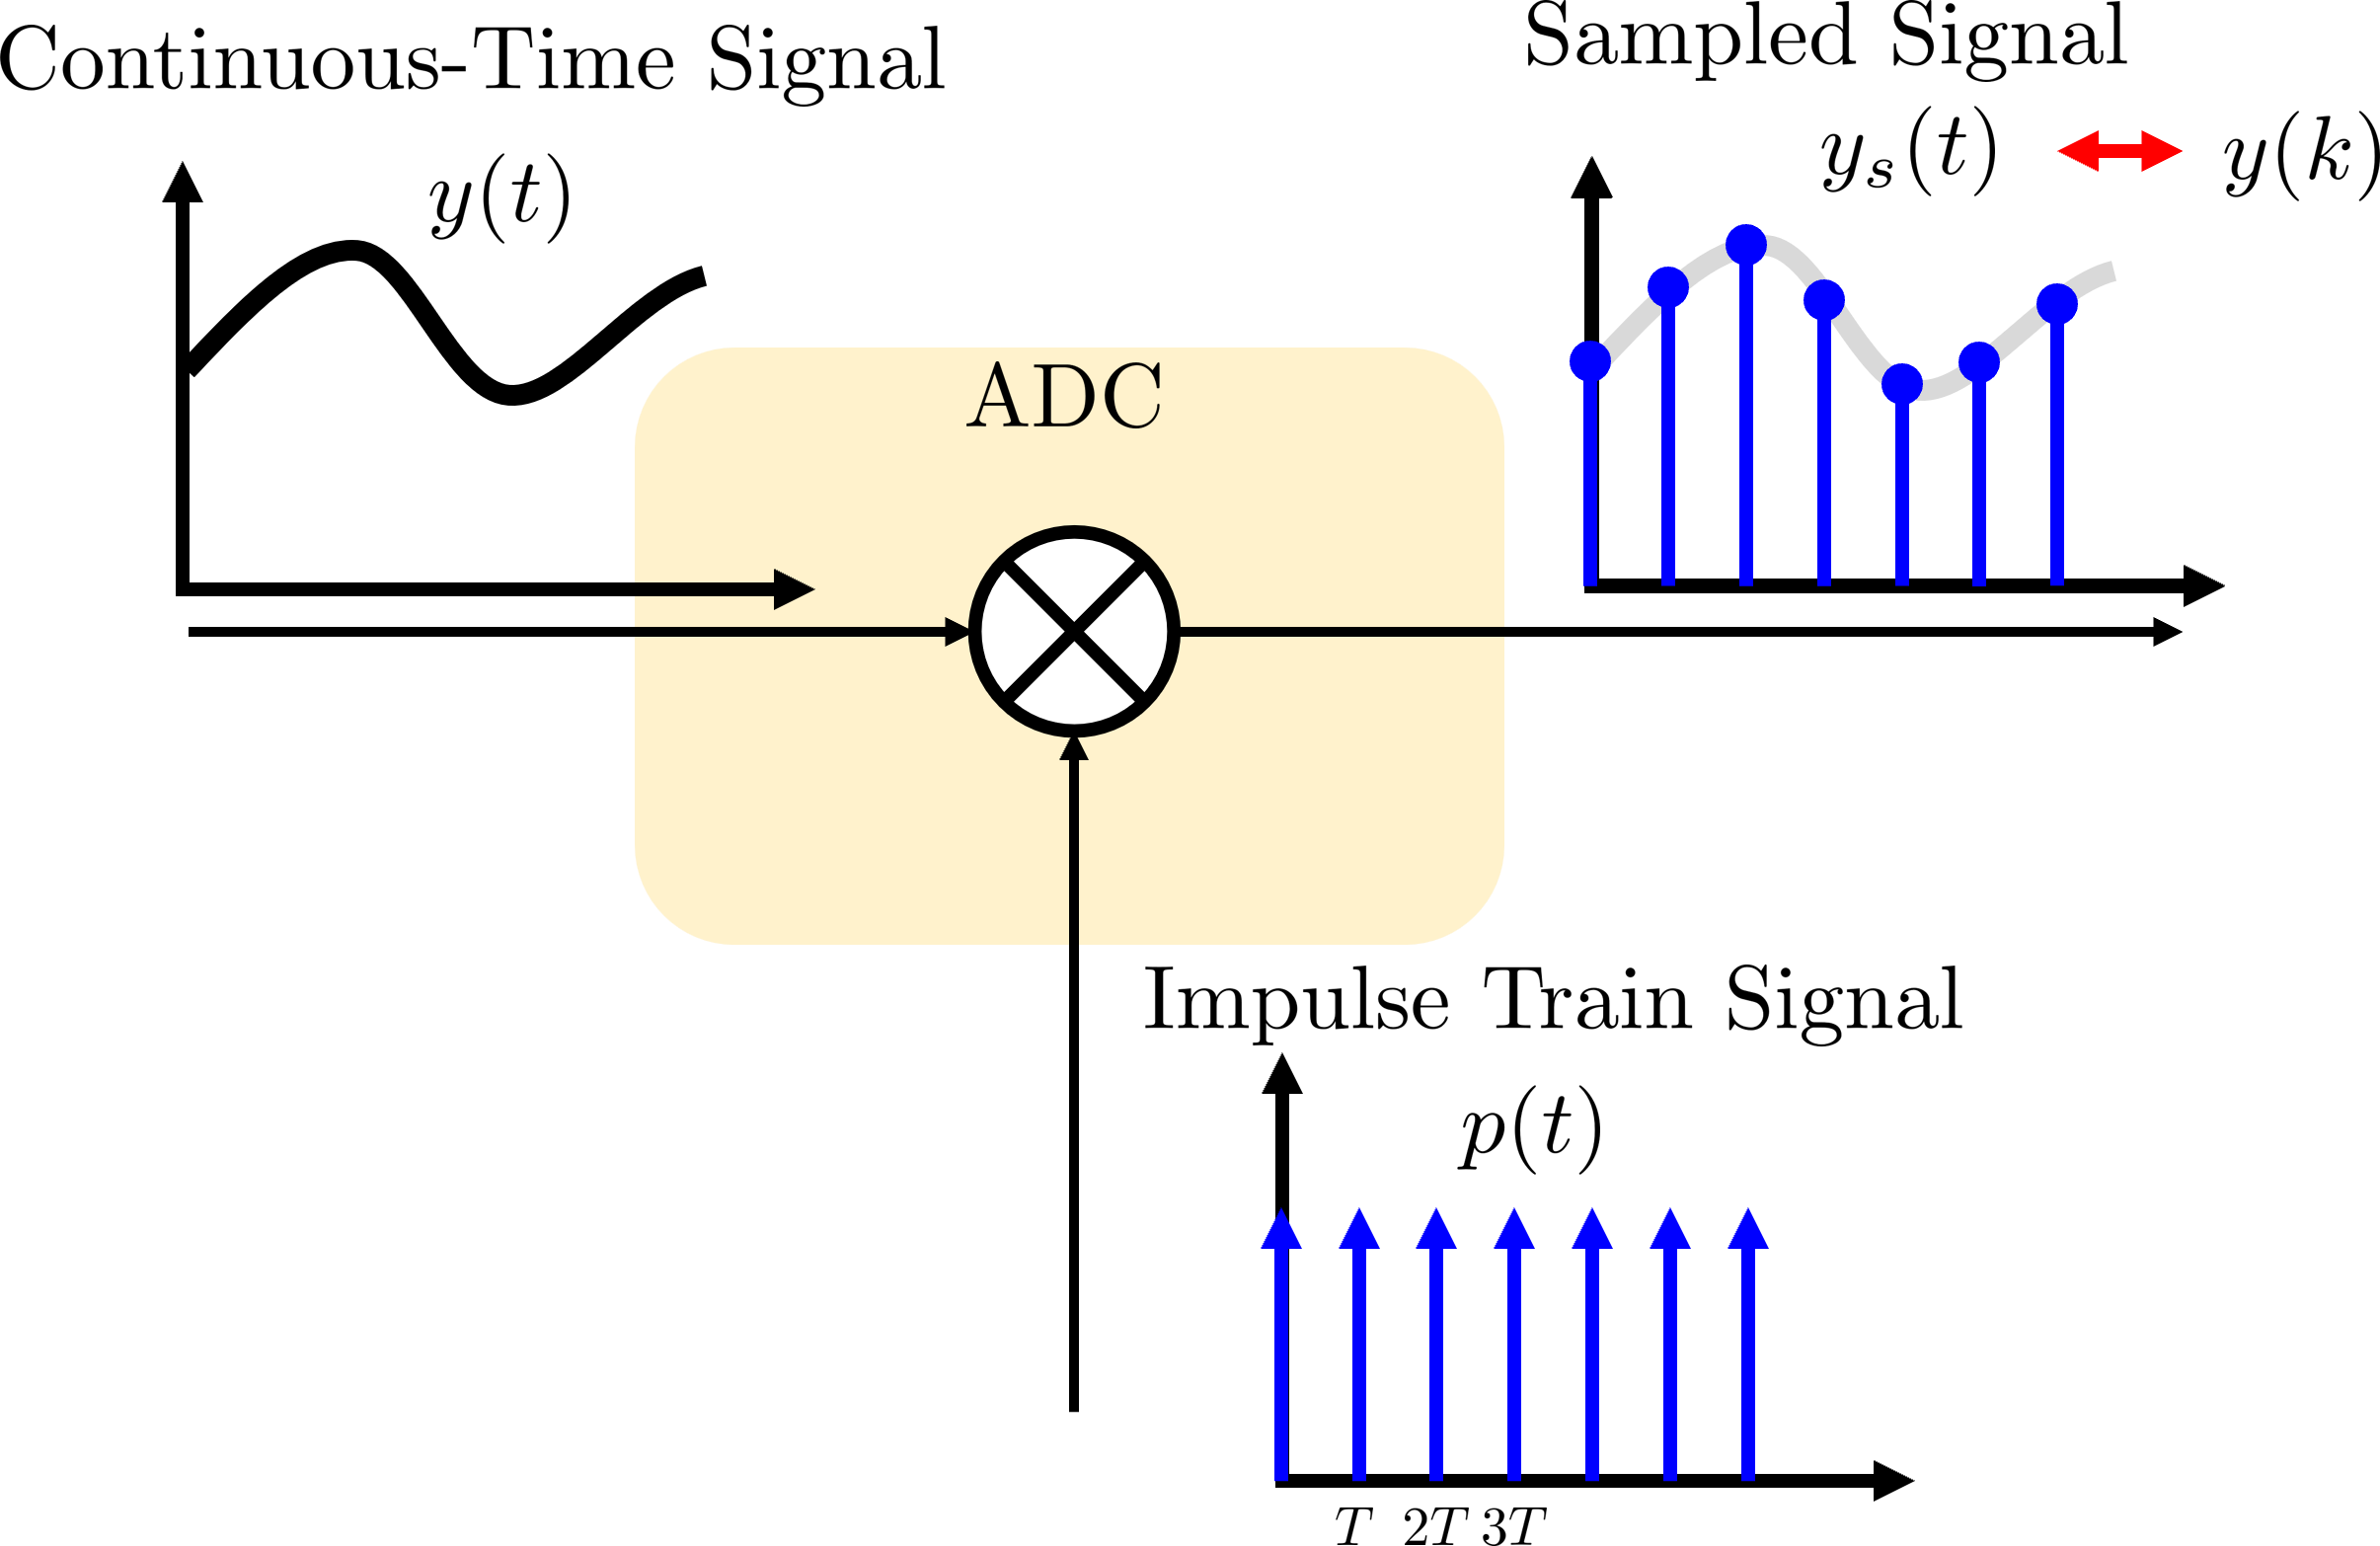
\includegraphics[width=10cm]{./FIG_Franklin/fig8-smc3.png}
	    \end{figure}
    \begin{enumerate}
    	\item Periodic Impulse Train: p(t) is periodic with period $T = 1/F_s$
    	\begin{align*}
    		p(t) = \sum_{k=-\infty}^{\infty} \delta(t-kT)
    	\end{align*}
     	\item Sampled Signal: we can consider $y_s(t)$ te be the analog equivalent to discrete-time signal $y(k)$ or $y(kT)$
    	\begin{align*}
    		y_s(t) &= y(t) \cdot p(t) = \sum_{k=-\infty}^{\infty} y(t)\delta(t-kT) = \sum_{k=-\infty}^{\infty} y(kT)\delta(t-kT)\\
    			&\leftrightarrow y(k) = y(kT)
    	\end{align*}
	\end{enumerate}   
    \newpage
    %!TEX root = ../main.tex
\setcounter{chapter}{7}
\setcounter{section}{0}
\section{Digitization}
\vspace{-8pt} \hrule \hrule \hrule \hrule \hrule  \vspace{12pt}
$\bigstar$ Nyquist–Shannon Sampling Theorem
\begin{enumerate}
	\item 간단하게, 아날로그 신호가 갖는 최대 주파수의 2배이상의 샘플링 주파수를 사용해야만 손실되는 정보없이 디지털 신호를 아날로그 신호로 복원할 수 있다.
	\item Nyquist freqeuncy(Folding Frequency): Sampling Frequency $F_s$의 절반 $F_{nyquist}=F_s/2$이며, 이는 신호의 최대 주파수 $F_{nyquist} \geq F_{max} $ 이어야 신호를 복원 할 수 있다. 
	\item Frequency Domain Analysis:
	\begin{align*}
	    \text{time-domain}& &&&&\text{frequency-domain}\\
		y_s(t) = y(t)\cdot p(t) & & \leftrightarrow & &Y_{s}(F) = &Y(F) \ast P(F) \\
		&&&&=& Y(F) \ast \frac{1}{T} \sum_{k =-\infty}^{\infty}\delta(F-kF_s)\\
		&&&&=& \frac{1}{T} \sum_{k =-\infty}^{\infty} Y(F-kF_{s})
	\end{align*}
\end{enumerate}

   
    \newpage
    %!TEX root = ../main.tex
\setcounter{chapter}{7}
\setcounter{section}{0}
\section{Digitization}
\vspace{-8pt} \hrule \hrule \hrule \hrule \hrule  \vspace{12pt}
	    \begin{figure}[!h]
	        \centering
	        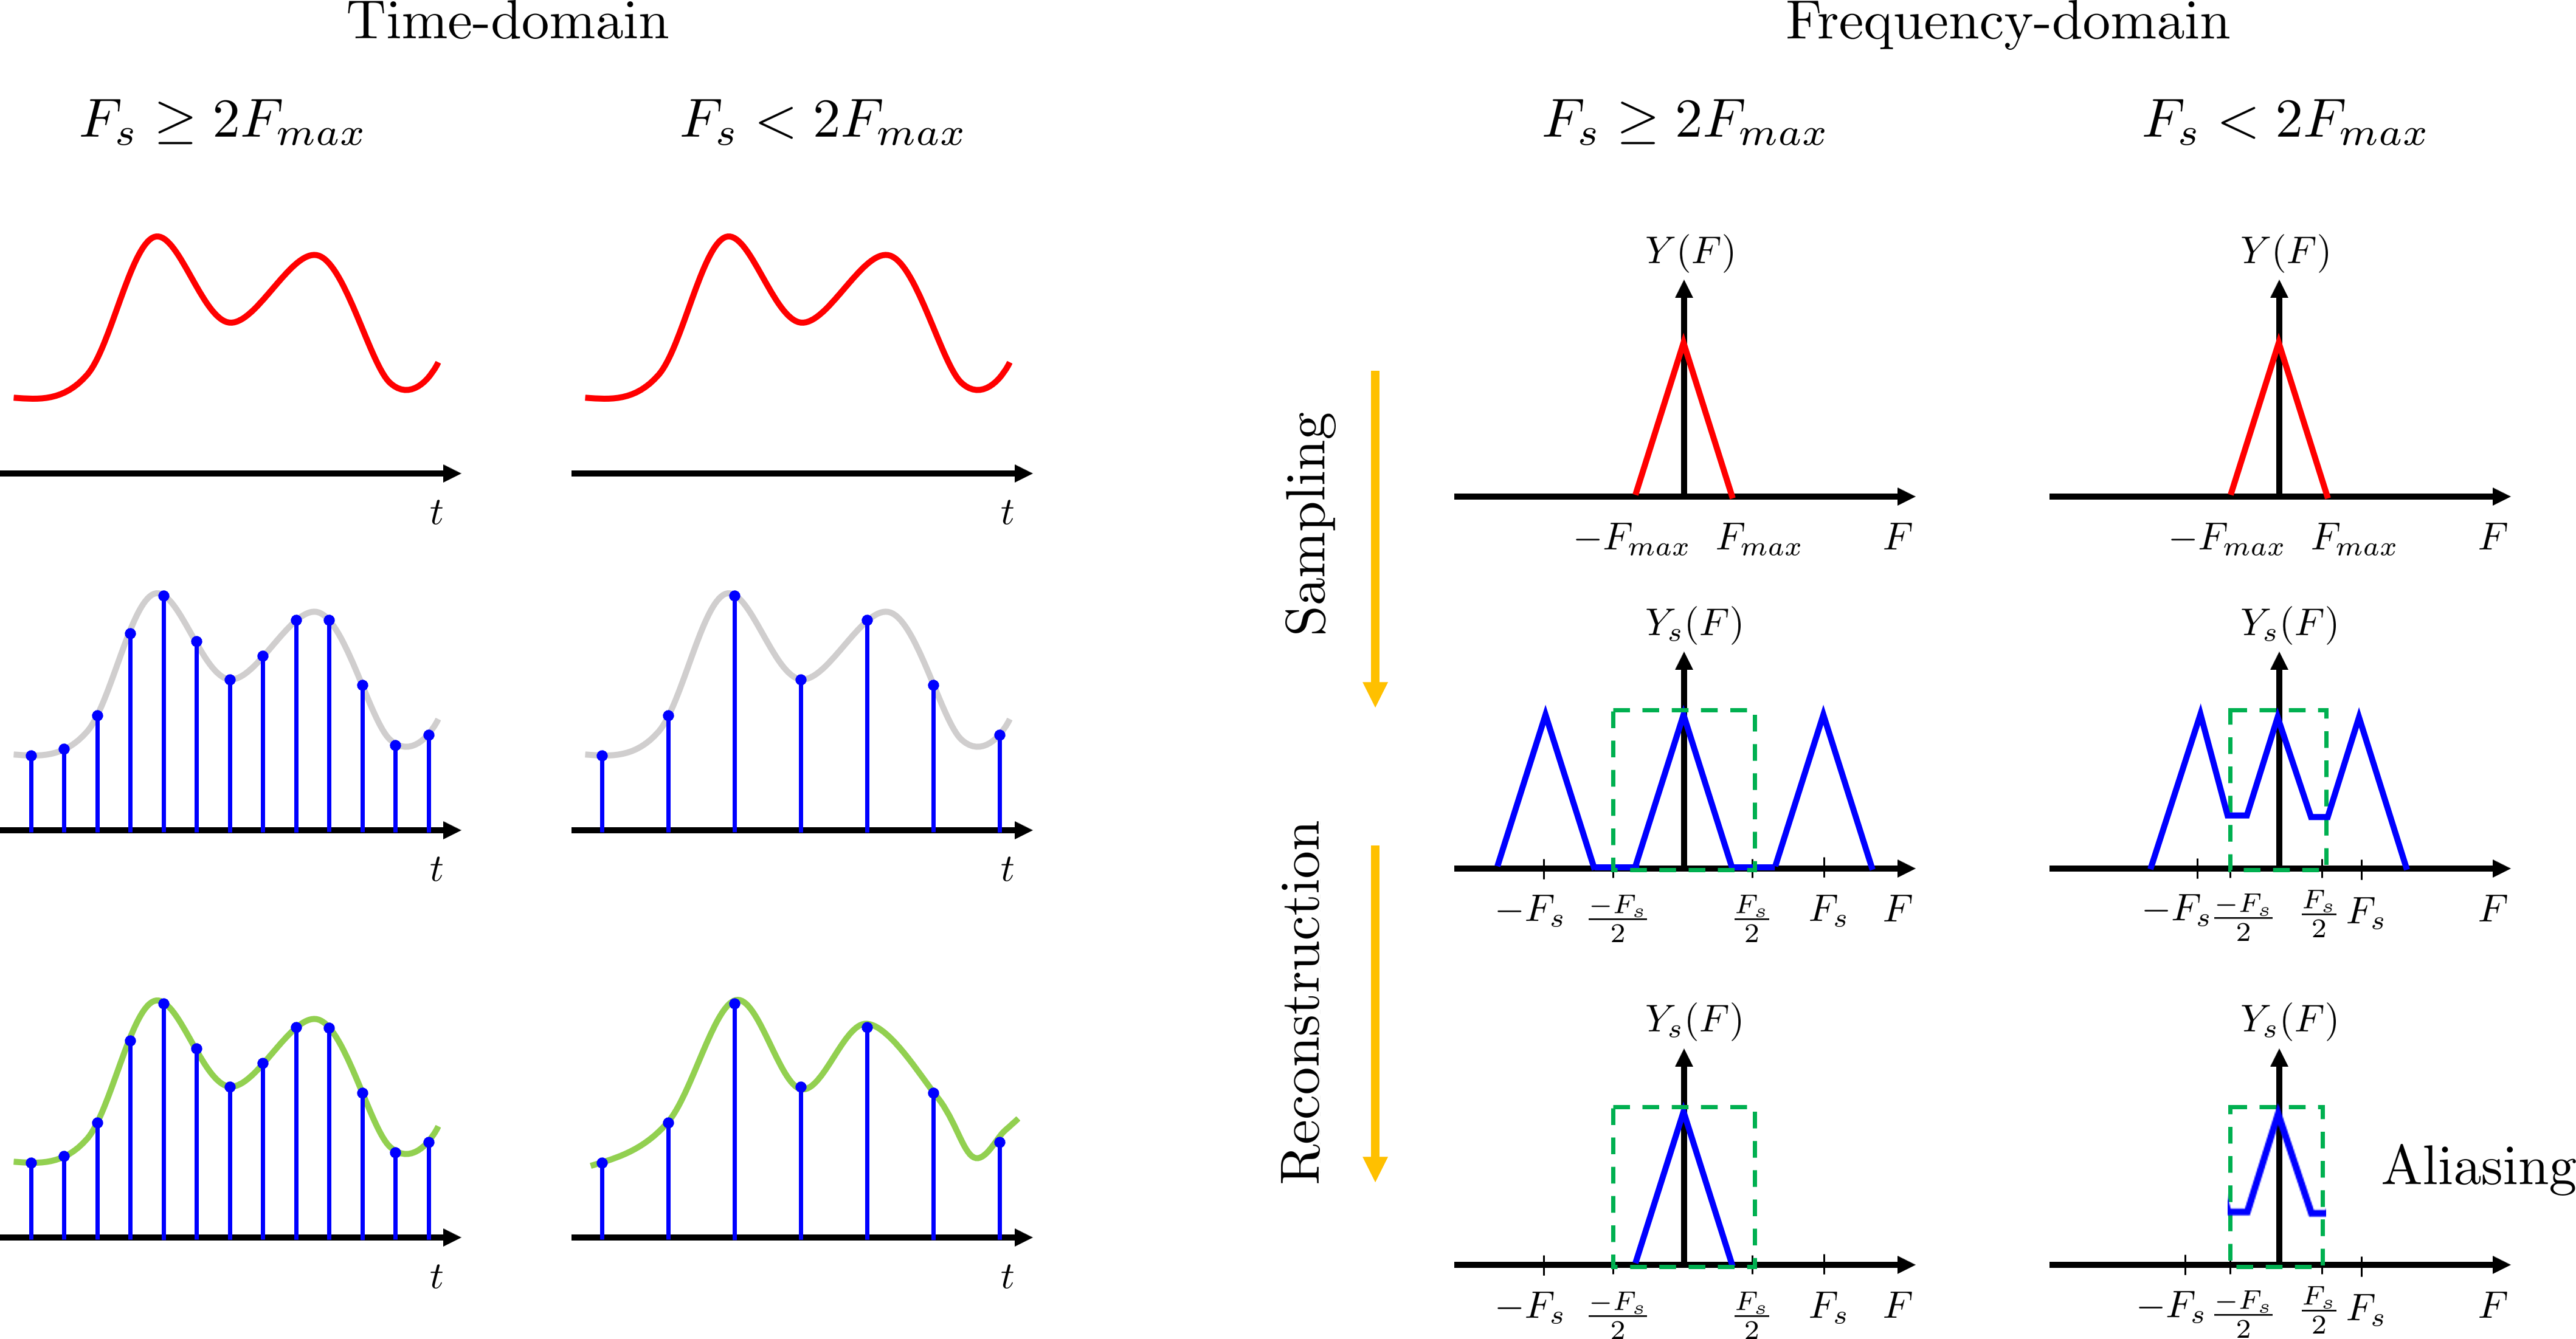
\includegraphics[width=24cm]{./FIG_Franklin/fig8-smc4.png}
	    \end{figure}   
    \newpage
    %!TEX root = ../main.tex
\setcounter{chapter}{7}
\setcounter{section}{0}
\section{Digitization}
\vspace{-8pt} \hrule \hrule \hrule \hrule \hrule  \vspace{12pt}

	    \begin{figure}[!h]
	        \centering
	        \includegraphics[width=24cm]{./FIG_Franklin/fig8-smc5.png}
	    \end{figure}
   
    \newpage    
    %!TEX root = ../main.tex
\setcounter{chapter}{7}
\setcounter{section}{1}
\section{Dynamic Analysis of Discrete Systems}
\vspace{-8pt} \hrule \hrule \hrule \hrule \hrule  \vspace{12pt}

% Please add the following required packages to your document preamble:
% \usepackage{booktabs}

\begin{table}[!hb]
\centering
\begin{tabular}{@{}|c|c|c|@{}}
\toprule
Condition                           & Discrete-Time                   & Continuous-Time   \\ \midrule
Periodic Signal                     & Discrete Fourier Series         & Fourier Series    \\ \midrule
Absolute Summable/Integrable Signal & Discrete-Time Fourier Transform & Fourier Transform \\ \midrule
Causal Signal                       & Unilateral $z$-Transfrom          & Unilateral Laplace Transform \\ \bottomrule
\end{tabular}
\end{table}
\begin{itemize}
	\item $z$-transform for discrete time systems $\leftrightarrow$ Laplace transform for continuous time systems. 
\item (8.2.1) $z$-Transform 
	\begin{enumerate}
		\item Laplace transform and its important property 
		\begin{align*}
			\mathcal{L} (f(t))&= F(s) = \int_{0^-}^{\infty} f(t) e^{-st} dt 
			&&&
			\mathcal{L}(\dot{f}(t)) &= sF(s) -f(0^{-})\\
			&&\Downarrow&
			\\
						\mathcal{L} (f(t))&= F(s) = \int_0^{\infty} f(t) e^{-st} dt 
			&&&
			\mathcal{L}(\dot{f}(t)) &= sF(s) \text{ } \text{ where $f(0^+) = 0$}
		\end{align*}
		$0^{-}$부터인 이유는 $f(t)$가 $\delta(t)$나 $\frac{d\delta(t)}{dt}$일때 Laplace Transform에 반영하기 위함, 이해를 돕기위해 정확한 정의는 아니지만 아래와 같은 정의 사용
	\end{enumerate}	
\end{itemize}

   
    \newpage    
    %!TEX root = ../main.tex
\setcounter{chapter}{7}
\setcounter{section}{0}
\section{Digitization}
\vspace{-8pt} \hrule \hrule \hrule \hrule \hrule  \vspace{12pt}

	\begin{enumerate}	
		\setcounter{enumi}{1}



	\item $z$-transform is defined by 
		\begin{align*}
			\mathcal{Z}(f(k)) &= F(z) = \sum_{k=0}^{\infty} f(k) z^{-k}  
			&&&
			\mathcal{Z} (f(k-1)) &=   \sum_{k=0}^{\infty} f(k-1) z^{-k}  
			\\
			&= f(0) + f(1) z^{-1} + f(2) z^{-2} + \cdots
			&&&
			&= f(-1) + f(0) z^{-1} + f(1) z^{-2} + f(2) z^{-3} + \cdots \\
			& &&& &= z^{-1} \left[  f(0) + f(1) z^{-1} + f(2) z^{-2} + \cdots \right] \\ 
			& &&& &= z^{-1} F(z) 
		\end{align*}
		where $f(k)$ is the sampled version of $f(t)$ and $z^{-1}$ represents one sample delay, and $f(-1) = 0$. \\

		Example) $x(0) = 0 ,x(1) = 1, x(2) = 2 ,x(3) = 3, x(4) = 4 $		\\
		\begin{flalign}
		 X(z) &= \sum_{k=0}^{\infty} x(k)z^{-k}\\
		      &=x(0) + x(1)z^{-1}+ x(2)z^{-2}+ x(3)z^{-3}+ x(4)z^{-4} \\
		      &= z^{-1}+2z^{-2}+3z^{-3}+4z^{-4}
        \end{flalign}
		\item Important property between LT and $z$-transform
		\begin{align*}
			z = e^{sT} ~~~~ \leftrightarrow~~~~ s = \frac{1}{T} \ln z  
		\end{align*}
		\item For example, the general second-order difference equation 
		\begin{align*}
			y(k) = -a_1 y(k-1) - a_2 y(k-2) + b_0 u(k) + b_1 u(k-1) + b_2 u(k-2) 
		\end{align*}
		can be converted from this form to the $z$-transform of the variables $y(k)$ and $u(k)$ by invoking above relations,
		\begin{align*}
			Y(z) = (-a_1 z^{-1} - a_2 z^{-2}) Y(z) + (b_0 + b_1 z^{-1} + b_2 z^{-2}) U(z) 
		\end{align*}
		now we have a discrete transfer function:
		\begin{align*}
			\frac{Y(z)}{U(z)} = \frac{b_0 + b_1 z^{-1} + b_2 z^{-2}}{1 + a_1 z^{-1} + a_2 z^{-2}} 
		\end{align*}
	\end{enumerate}	
   
    \newpage    
    %!TEX root = ../main.tex
\setcounter{chapter}{7}
\setcounter{section}{1}
\section{Dynamic Analysis of Discrete Systems}
\vspace{-8pt} \hrule \hrule \hrule \hrule \hrule  \vspace{12pt}

	\begin{enumerate}	
		\setcounter{enumi}{3}
		\item For example, the general second-order difference equation 
		\begin{align*}
			y(k) = -a_1 y(k-1) - a_2 y(k-2) + b_0 u(k) + b_1 u(k-1) + b_2 u(k-2) 
		\end{align*}
		can be converted from this form to the $z$-transform of the variables $y(k)$ and $u(k)$ by invoking above relations,
		\begin{align*}
			Y(z) &= -a_1 z^{-1} Y(z) -a_2 z^{-2} Y(z) + b_0 U(z) + b_1 z^{-1} U(z) + b_2 z^{-2} U(z)\\
			     &= (-a_1 z^{-1} - a_2 z^{-2}) Y(z) + (b_0 + b_1 z^{-1} + b_2 z^{-2}) U(z) 
		\end{align*}
		now we have a discrete transfer function:
		\begin{align*}
			Y(z) - (-a_1 z^{-1} - a_2 z^{-2}) Y(z) &= (b_0 + b_1 z^{-1} + b_2 z^{-2}) U(z) \\
			(1 +a_1 z^{-1} + a_2 z^{-2}) Y(z) &= (b_0 + b_1 z^{-1} + b_2 z^{-2}) U(z) \\
			\frac{Y(z)}{U(z)} = \frac{b_0 + b_1 z^{-1} + b_2 z^{-2}}{1 + a_1 z^{-1} + a_2 z^{-2}} 
		\end{align*}

	\end{enumerate}	   
    \newpage   
    %!TEX root = ../main.tex
\setcounter{chapter}{7}
\setcounter{section}{1}
\section{Dynamic Analysis of Discrete Systems}
\vspace{-8pt} \hrule \hrule \hrule \hrule \hrule  \vspace{12pt}

\begin{itemize}	

\item (8.2.1) $z$-Transform 
	\begin{enumerate}
		\item See the Table 8.1 for understanding between $z$-transform and LT
		\begin{table}[h]
		\centering
			\begin{tabular}{c||c||c|c} 
				\hline \hline 
				$F(s)$ & $f(kT)$ & $F(z)$ & \\ \hline
				- & $\delta(kT)$ & 1 & 1 \\
				- & $\delta(kT-k_0 T)$ & $z^{-k_0}$ & $z^{-k_0}$ \\
				$\frac{1}{s}$ & $1(kT)$ & $\frac{z}{z-1}$ & $\frac{1}{1-z^{-1}}$ \\
				$\frac{1}{s^2}$ & $kT$ & $\frac{Tz}{(z-1)^2}$ & $\frac{Tz^{-1}}{(1-z^{-1})^2} $ \\
				$\frac{1}{s+a}$ & $e^{-akT}$ & $\frac{z}{z-e^{-aT}}$ & $\frac{1}{1-e^{-aT}z^{-1}}$ \\
				$\frac{1}{s(s+a)}$ & $1-e^{-akT}$ & $\frac{z(1-e^{-aT})}{(z-1)(z-e^{-aT})}$ & $\frac{z^{-1}(1-e^{-aT})}{(1-z^{-1})(1-e^{-aT} z^{-1})}$ \\
				$\frac{a}{s^2+a^2}$ & $\sin a kT$ & $\frac{z \sin aT}{z^2-(2\cos aT)z +1}$ & $\frac{z^{-1}  \sin aT}{1-(2\cos aT)z^{-1} + z^{-2}}$ \\
				$\frac{s}{s^2+a^2}$ & $\cos a kT$ & $\frac{z(z- \cos aT)}{z^2-(2\cos aT)z +1}$ & $\frac{(1- z^{-1}\cos aT )}{1-(2\cos aT)z^{-1} +z^{-2}}$ \\
				\hline \hline 
			\end{tabular}
		\end{table}
		\item For parts of Table, we have
		\begin{align*}
			\mathcal{Z}(\delta(kT)) &=\sum_{k=0}^{k=\infty}\delta(kT)z^{-k}= \delta(0 \cdot T) + \delta(1 \cdot T)z^{-1} + \cdots  = 1  + 0 z^{-1} + 0 z^{-2} + \cdots = 1  \\  
			\mathcal{Z}(\delta(k-k_0T)) &= 0  + 0 z^{-1} +  \cdots + 1 z^{-k_0} + \cdots +  = z^{-k_0}  \\  
			\mathcal{Z}(1(kT)) &= 1 + z^{-1} + z^{-2} + \cdots = \frac{1}{1-z^{-1}} = (1-z^{-1})^{-1}  \\
			\mathcal{Z}(e^{-akT}) &= 1 + e^{-aT} z^{-1} + e^{-2aT} z^{-2} + \cdots = \frac{1}{1-e^{-aT}z^{-1}} \\
		\end{align*}
	\end{enumerate}

\end{itemize}			   
    \newpage  
          %!TEX root = ../main.tex
\setcounter{chapter}{7}
\setcounter{section}{0}
\section{Digitization}
\vspace{-8pt} \hrule \hrule \hrule \hrule \hrule  \vspace{12pt}
   
    \newpage    
    %!TEX root = ../main.tex
\setcounter{chapter}{7}
\setcounter{section}{1}
\section{Dynamic Analysis of Discrete Systems}
\vspace{-8pt} \hrule \hrule \hrule \hrule \hrule  \vspace{12pt}


				\begin{align*}
							\mathcal{Z}(1-e^{-akT}) &= \mathcal{Z}(1) - \mathcal{Z}(e^{-akT}) = \frac{1}{1-z^{-1} } -  \frac{1}{1-e^{-aT}z^{-1}}\\
							                        & = \frac{z^{-1}-e^{-aT}z^{-1}}{(1-z^{-1})(1-e^{-aT}z^{-1})} =  \frac{z^{-1}(1-e^{-aT})}{(1-z^{-1})(1-e^{-aT}z^{-1})} \\
				\end{align*}
				\begin{align*}
					\mathcal{Z}(\cos(-akT))  &= \mathcal{Z}(\frac{e^{jakT}+e^{-jakT}}{2}) =\frac{\mathcal{Z}(e^{jakT})}{2} +\frac{\mathcal{Z}(e^{-jakT})}{2}  \\
					 & = \frac{1}{2} \cdot \frac{1}{1-e^{jaT}z^{-1}}  + \frac{1}{2} \cdot \frac{1}{1-e^{-jaT}z^{-1}} \\
					 & = \frac{(1- z^{-1}\cos aT )}{1-(2\cos aT)z^{-1} +z^{-2}}
				\end{align*}

				\begin{align*}
					\mathcal{Z}(\sin(-akT)) = ? , \mathcal{Z}(\sinh(-akT)) = ? , \mathcal{Z}(\cosh(-akT))= ?
				\end{align*}

	   
    \newpage    
            %!TEX root = ../main.tex
\setcounter{chapter}{7}
\setcounter{section}{0}
\section{Digitization}
\vspace{-8pt} \hrule \hrule \hrule \hrule \hrule  \vspace{12pt}
   
    \newpage    
    %!TEX root = ../main.tex
\setcounter{chapter}{7}
\setcounter{section}{0}
\section{Digitization}
\vspace{-8pt} \hrule \hrule \hrule \hrule \hrule  \vspace{12pt}
   
    \newpage  
    %!TEX root = ../main.tex
\setcounter{chapter}{7}
\setcounter{section}{0}
\section{Digitization}
\vspace{-8pt} \hrule \hrule \hrule \hrule \hrule  \vspace{12pt}
   
    \newpage        
    %!TEX root = ../main.tex
\setcounter{chapter}{7}
\setcounter{section}{1}
\section{Dynamic Analysis of Discrete Systems}
\vspace{-8pt} \hrule \hrule \hrule \hrule \hrule  \vspace{12pt}
	\begin{enumerate}
		\setcounter{enumi}{3}
\item See Fig. 8.4, and it shows the mapping of lines of constant damping $\zeta$ and natural frequency $\omega_n$ from $s$-plane to the upper half of the $z$-plane, using $z = e^{sT}$. 

		\begin{figure}[h]
		    \centering
			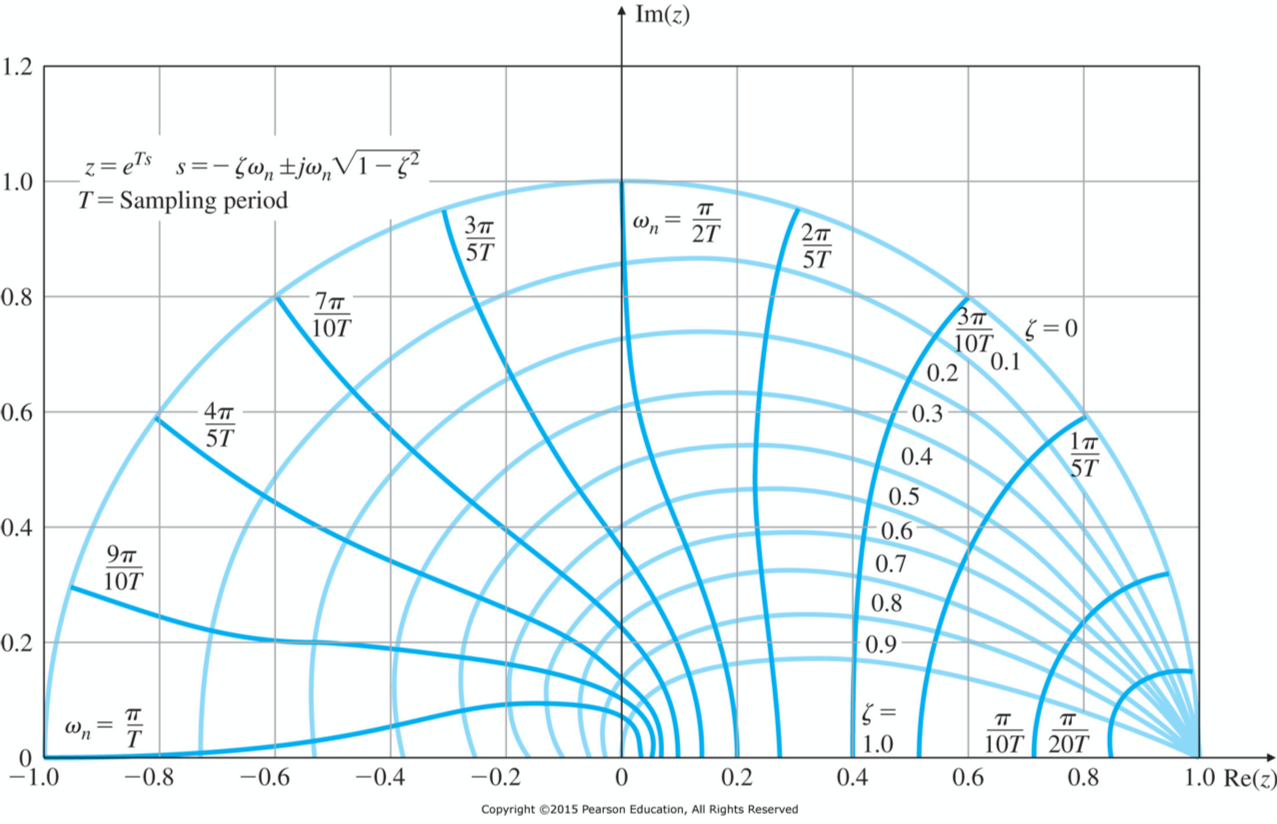
\includegraphics[width=7cm]{./FIG_Franklin/fig8-4.png}\\
			\url{http://controlsystemsacademy.com/0003/0003.html}
		\end{figure}
		\begin{enumerate}
			\item The stability boundary $s= 0 \pm j\omega$ becomes the unit circle $|z| =1$ in the $z$-plane; inside the unit circle is stable, outside is unstable\\
			s-plane에서의 stability boundary는 imaginary축 $s = \pm j\omega$ 인데 z-plane에서의 stability boundary는 unit circle $|z|=e^{sT}|_{s=\pm j \omega }= 1 $이 된다.
			\item The small vicinity around $z=+1$ in the $z$-plane is essentially identical to the vicinity around the origin $s=0$, in the $s$-plane.\\
			z-plane 에서의 $z=1$근방은 s-plane에서의 $s=0$ 근방과 같다.
			\item The $z$-plane locations give response information normalized to the sample rate rather than to time as in the $s$-plane. \\
			z-plane 에서의 response information은 s-plane에서와 같이 시간에 대한 정보가 아닌, sample rate로 normalized된 정보를 제공한다.
			\newpage
			\item The negative real $z$-axis always represents a frequency of $\omega_s/2$, where $\omega_s = 2\pi/T = $ circular sample rate in radians per second.\\
			 $\omega_s$가  $2\pi/T$ 일때 음의 $z$축은 $\omega_s/2$로 표현된다.
			\item Vertical lines in the left half of the $s$-plane (the constant real part of $s$) map into \emph{circles} within the unit circle of the $z$-plane \\
			s-plane에서의 좌반면은 z-plane에서의 unit circle 내부로 매핑된다.
			\item Horizontal lines in the $s$-plane (the constant imaginary part of $s$) map into \emph{radial lines} in the $z$-plane. \\
			s-plane에서의 수평선은 z-plane에서의 radial line들로 매핑된다.
			\item Frequencies greater than $\omega_s/2$, called the Nyquist frequency, appear in the $z$-plane on the top of corresponding lower frequencies because of the circular characteristics of $e^{sT}$. This overlap is called \emph{aliasing} or folding.  
		\end{enumerate} 
		\item As a result, it is necessary to sample at least twice as fast as a signal's highest frequency component in order to represent that signal with the samples. 

	\end{enumerate}   
    \newpage        
    %!TEX root = ../main.tex
\setcounter{chapter}{7}
\setcounter{section}{1}
\section{Dynamic Analysis of Discrete Systems}
\vspace{-8pt} \hrule \hrule \hrule \hrule \hrule  \vspace{12pt}
\begin{itemize}
\item (8.2.4) Final Value Theorem 
	\begin{enumerate}
		\item Discrete final value theorem is 
		\begin{align*}
			\lim_{t \rightarrow \infty} x(t) = x_{ss} &= \lim_{s \rightarrow 0} sX(s) &&&
			\lim_{k \rightarrow \infty} x(k) = x_{ss} &= \lim_{z \rightarrow 1} (1-z^{-1}) X(z) 
		\end{align*}
		if all the poles of $(1-z^{-1}) X(z)$ are inside the unit circle. 
		\item For example, to find the DC gain of the TF
		\begin{align*}
			G(z) = \frac{X(z)}{U(z)} = \frac{0.58(1+z)}{z+0.16} 
		\end{align*}
		we let $u(k) =1 $ for $k \geq 0$, so that 
		\begin{align*}
			U(z) = \frac{1}{1-z^{-1}} ~~~\text{and} ~~~ X(z) = \frac{0.58(1+z)}{(1-z^{-1})(z+0.16)}
		\end{align*}

		Applying the final value theorem yields 
		\begin{align*}
			x_{ss} &= \lim_{z \rightarrow 1} (1-z^{-1}) X(z) = \frac{0.58 \cdot 2}{1+0.16} = 1
		\end{align*}
		so the DC gain of $G(z)$ is unity. 
	\end{enumerate}
\end{itemize}	   
    \newpage        
    %!TEX root = ../main.tex
\setcounter{chapter}{7}
\setcounter{section}{1}
\section{Dynamic Analysis of Discrete Systems}
\vspace{-8pt} \hrule \hrule \hrule \hrule \hrule  \vspace{12pt}   
    \newpage        
    %!TEX root = ../main.tex
\setcounter{chapter}{7}
\setcounter{section}{0}
\section{Digitization}
\vspace{-8pt} \hrule \hrule \hrule \hrule \hrule  \vspace{12pt}
   
    \newpage        
    %!TEX root = ../main.tex
\setcounter{chapter}{7}
\setcounter{section}{2}
\section{Design using Discrete Equivalents}
\vspace{-8pt} \hrule \hrule \hrule \hrule \hrule  \vspace{12pt}

\begin{enumerate}
	\setcounter{enumi}{1}
		\item Taking $z$-transform, 
		\begin{align*}
			\frac{U(z)}{E(z)} = \frac{T}{2} \frac{1+z^{-1}}{1-z^{-1}} = \frac{1}{\frac{2}{T} \frac{1-z^{-1}}{1+z^{-1}} }
		\end{align*}
		\item In fact, the Tustin's method approximates $z = e^{sT}$ as follows:
		\begin{align*}
			s \approx  \frac{2}{T} \frac{1-z^{-1}}{1+z^{-1}}
		\end{align*}
		where it can be derived from the Taylor's series expansions as follows:
		\begin{align*}
			z &= e^{sT} = \frac{e^{\frac{sT}{2}}}{e^{-\frac{sT}{2}}} 
			= \frac{1 + \frac{sT}{2} + \frac{s^2T^2}{2^2} + \cdots}{1 - \frac{sT}{2} + \frac{s^2T^2}{2^2} - \cdots} \approx  \frac{1 + \frac{sT}{2}}{1 - \frac{sT}{2}}  = \frac{2+sT}{2-sT} 
			~~~~~\rightarrow~~~~~ s \approx  \frac{2}{T} \frac{z-1}{z+1} = \frac{2}{T} \frac{1-z^{-1}}{1+z^{-1}}
		\end{align*}

\end{enumerate}   
    \newpage        
    %!TEX root = ../main.tex
\setcounter{chapter}{7}
\setcounter{section}{0}
\section{Digitization}
\vspace{-8pt} \hrule \hrule \hrule \hrule \hrule  \vspace{12pt}
   
    \newpage        
    %!TEX root = ../main.tex
\setcounter{chapter}{7}
\setcounter{section}{2}
\section{Design using Discrete Equivalents}
\vspace{-8pt} \hrule \hrule \hrule \hrule \hrule  \vspace{12pt}
\begin{enumerate}
	\setcounter{enumi}{4}
	\item (Example 8.1) Determine the difference equation with a sample rate of 25 times bandwidth using Tustin's approximation. 
		\begin{align*}
			D_c(s) = 10 \frac{s/2+1}{s/10+1} ~~~~ \text{Lead compensator} 
		\end{align*}
		Since the bandwidth is approximately $\omega_{bd} = 10[rad/s]$, the sampling rate should be
		\begin{align*}
			\omega_s = 25 \times \omega_{bd} = 250 [rad/s] ~~~~ \rightarrow~~~~~ f_s = \frac{\omega_s}{2\pi} \approx 40[Hz] ~~~~\rightarrow~~~~ T = \frac{1}{f_s} = \frac{1}{40} = 0.025[s]
		\end{align*}
		The discrete TF can be obtained as 
		\begin{align*}
			D_d(z) &= 10 \frac{\frac{1}{T} \frac{1-z^{-1}}{1+z^{-1}}+1}{\frac{1}{5T} \frac{1-z^{-1}}{1+z^{-1}}+1} =  10 \frac{5(1-z^{-1})+ 5T(1+z^{-1})}{(1-z^{-1})+ 5T(1+z^{-1})} \\
			&= 50 \frac{(1+T) - (1-T)z^{-1}}{(1+5T) - (1-5T)z^{-1}} 
			= 50 \frac{1.025 - 0.975z^{-1}}{1.125 - 0.875z^{-1}} 
			= \frac{45.556 - 43.333 z^{-1}}{1 - 0.778z^{-1}}
		\end{align*}
		Finally, the difference equation is 
		\begin{align*}
			u(k) &= 0.778 u(k-1) + 45.556 [ e(k) -  0.951 e(k-1) ]
		\end{align*}
\end{enumerate}		   
    \newpage        
    %!TEX root = ../main.tex
\setcounter{chapter}{7}
\setcounter{section}{2}
\section{Design using Discrete Equivalents}
\vspace{-8pt} \hrule \hrule \hrule \hrule \hrule  \vspace{12pt}
Matlab Code
\begin{lstlisting}
clc;clear all; format compact; close all;
s=tf('s');
Dc = 10*(s/2+1)/(s/10+1)
Ts = 0.025;
Dz = c2d(Dc,Ts,'tustin');
[num,den]=tfdata(Dz);
Dz = tf(num,den,Ts,"Variable","z^-1")
figure(1)
step(Dc);
hold on;
step(Dz);
\end{lstlisting}
\url{http://controlsystemsacademy.com/0003/0003.html}\\
Result
\begin{lstlisting}
% Dc =
%   100 s + 200
%   -----------
%    2 s + 20
% Dz =
%   45.56 - 43.33 z^-1
%   ------------------
%    1 - 0.7778 z^-1
% Sampling Time: 0.025 seconds
\end{lstlisting}
\newpage
\begin{figure}[h]
	\centering
	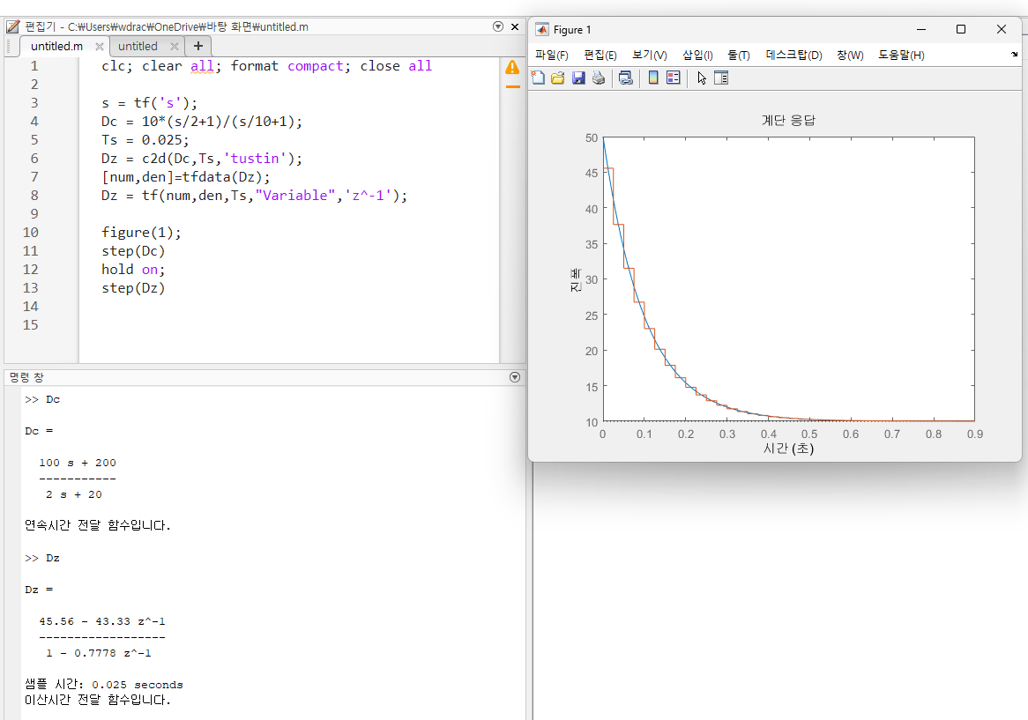
\includegraphics[width=20cm]{./FIG_Franklin/fig8-smc6.png}
\end{figure}   
    \newpage     
    %!TEX root = ../main.tex
\setcounter{chapter}{7}
\setcounter{section}{0}
\section{Digitization}
\vspace{-8pt} \hrule \hrule \hrule \hrule \hrule  \vspace{12pt}
   
    \newpage      
    %!TEX root = ../main.tex
\setcounter{chapter}{7}
\setcounter{section}{0}
\section{Digitization}
\vspace{-8pt} \hrule \hrule \hrule \hrule \hrule  \vspace{12pt}
   
    \newpage      

    %!TEX root = ../main.tex
\setcounter{chapter}{7}
\setcounter{section}{0}
\section{Digitization}
\vspace{-8pt} \hrule \hrule \hrule \hrule \hrule  \vspace{12pt}
   
    \newpage              
    %!TEX root = ../main.tex
\setcounter{chapter}{7}
\setcounter{section}{0}
\section{Digitization}
\vspace{-8pt} \hrule \hrule \hrule \hrule \hrule  \vspace{12pt}
   
    \newpage              
    %!TEX root = ../main.tex
\setcounter{chapter}{7}
\setcounter{section}{2}
\section{Design using Discrete Equivalents}
\vspace{-8pt} \hrule \hrule \hrule \hrule \hrule  \vspace{12pt}
\begin{enumerate}
	\setcounter{enumi}{4}
	\item (Example 8.2) Determine the difference equation with a sample period $T=0.025[s]$ using ZOH approximation. 
		\begin{align*}
			D_c(s) = 10 \frac{s/2+1}{s/10+1} = 10 \frac{5s+10}{s+10}
		\end{align*}
		The discrete TF using ZOH  is 
		\begin{align*}
			D_d(z) = 10 (1-z^{-1}) \mathcal{Z} \left( \frac{5s+10}{s(s+10)} \right)
			&= 10 (1-z^{-1}) \mathcal{Z} \left(  \frac{5}{s+10} + \frac{10}{s(s+10)} \right) \\
			&= 10 (1-z^{-1})  \left( \frac{5}{1-e^{-0.25}z^{-1}} + \frac{z^{-1}(1-e^{-0.25})}{(1-z^{-1})(1-e^{-0.25}z^{-1})} \right) \\
			&=  10 (1-z^{-1})  \left(  \frac{5(1-z^{-1}) + z^{-1}(1-e^{-0.25})}{(1-z^{-1})(1-e^{-0.25}z^{-1})} \right) \\
			&=   \frac{50 - 47.79z^{-1}}{1 - 0.779z^{-1}} 
		\end{align*}
	where $\mathcal{Z} \left\{ \frac{1}{s+10} \right\} = \frac{1}{1-e^{-10T}z^{-1}}$ with  $e^{-10T} = e^{-0.25}=0.779$. Or, 
		\begin{align*}
			D_d(z) = 10 (1-z^{-1}) \mathcal{Z} \left( \frac{5s+10}{s(s+10)} \right)
			&= 10 (1-z^{-1}) \mathcal{Z} \left(  \frac{1}{s} + \frac{4}{s+10} \right) \\
			&= 10 (1-z^{-1})  \left( \frac{1}{1-z^{-1}} + \frac{4}{1-e^{-0.25}z^{-1}} \right) \\
			&=  10 (1-z^{-1})  \left(  \frac{(1-e^{-0.25}z^{-1})+ 4(1-z^{-1})}{(1-z^{-1})(1-e^{-0.25}z^{-1})} \right) \\
			&=   \frac{50 - 47.79z^{-1}}{1 - 0.779z^{-1}} 
		\end{align*}
		Finally, the difference equation is 
		\begin{align*}
			u(k) &= 0.779 u(k-1) + 50 e(k) - 47.79 e(k-1) \\
			&= 0.779 u(k-1) + 50 [ e(k) -  0.956 e(k-1) ]
		\end{align*}

	\end{enumerate}
   
    \newpage              
    %!TEX root = ../main.tex
\setcounter{chapter}{7}
\setcounter{section}{0}
\section{Digitization}
\vspace{-8pt} \hrule \hrule \hrule \hrule \hrule  \vspace{12pt}
   
    \newpage              
    %!TEX root = ../main.tex
\setcounter{chapter}{7}
\setcounter{section}{2}
\section{Design using Discrete Equivalents}
\vspace{-8pt} \hrule \hrule \hrule \hrule \hrule  \vspace{12pt}
\begin{itemize}
	\item (8.3.3) Matched Pole-Zero (MPZ) Method 
	\begin{enumerate}
		\item Another digitization method, called the matched pole-zero (MPZ) method, is suggested by matching the poles and zeros between $s$ and $z$ planes, using $z = e^{sT}$. 
		\item Because physical systems often have more poles than zeros, it is useful to arbitrarily add zeros at $z=-1$, resulting in a $(1+z^{-1})$ term in $D_d(z)$.
		\begin{enumerate}
			\item Map poles and zeros according to the relation $z = e^{sT}$
			\item If the numerator is of lower order than the denominator, add powers of $(1+z^{-1})$ to the numerator until numerator and denominator are of equal order.
			\item Set the DC or low frequency gain of $D_d(z)$ equal to that of $D_c(s)$.
		\end{enumerate}
		\item For example, the MPZ approximation  
		\begin{align*}
			D_c(s) &= K_c \frac{s+a}{s+b} &&& D_d(z) &= K_d \frac{1-e^{-aT}z^{-1}}{1-e^{-bT}z^{-1}}
		\end{align*}
		where $K_d$ is found by the DC-gain 
		\begin{align*}
			\lim_{s \rightarrow 0} D_c(s) = K_c \frac{a}{b} ~~~~\rightleftarrows~~~~~ 
			\lim_{z \rightarrow 1} D_d(z) = K_d \frac{1-e^{-aT}}{1-e^{-bT}} 
		\end{align*} 
		Thus the result is
		\begin{align*}
			K_d = K_c \frac{a}{b} \left( \frac{1-e^{-bT}}{1-e^{-aT}} \right) 
		\end{align*}
	\end{enumerate}

\end{itemize}		   
    \newpage              
    %!TEX root = ../main.tex
\setcounter{chapter}{7}
\setcounter{section}{0}
\section{Digitization}
\vspace{-8pt} \hrule \hrule \hrule \hrule \hrule  \vspace{12pt}
   
    \newpage              
    %!TEX root = ../main.tex
\setcounter{chapter}{7}
\setcounter{section}{2}
\section{Design using Discrete Equivalents}
\vspace{-8pt} \hrule \hrule \hrule \hrule \hrule  \vspace{12pt}
\begin{enumerate}
	\setcounter{enumi}{4}
		\item (Example 8.3) Design a digital controller to have a closed-loop natural frequency $\omega_n = 0.3$ and a damping ratio $\zeta = 0.7$, another real pole at $s=-1.58$, using MPZ digitization
		\begin{align*}
			G(s) = \frac{1}{s^2}
		\end{align*}
		Let us assume that the lead compensator is used
		\begin{align*}
			D_c(s) = K_c \frac{s+b}{s+a} 
		\end{align*}
		Then, we have the characteristic equation
		\begin{align*}
			1+G(s) D_c(s) &= 1 + K_c \frac{s+b}{s^2(s+a)}  = s^3 + as^2 + K_c s + K_c b \\
			\alpha_c(s) &= (s^2 + 2 \zeta \omega_n s + {\omega_n }^2)(s- p)\\
						&= (s^2 + 0.42s + 0.09)(s+1.58) = s^3 + 2s^2 + 0.7536s + 0.1422
		\end{align*}
	    with $a=2$, $b=0.19$, and $K_c = 0.7536$. Now we have the lead compensator: 
		\begin{align*}
			D_c(s) = 0.7536 \frac{s+0.19}{s+2} ~~~~\rightarrow~~~~
			D_c(s) = 0.81 \frac{s+0.2}{s+2}
		\end{align*}

	\end{enumerate}   
    \newpage              
    %!TEX root = ../main.tex
\setcounter{chapter}{7}
\setcounter{section}{2}
\section{Design using Discrete Equivalents}
\vspace{-8pt} \hrule \hrule \hrule \hrule \hrule  \vspace{12pt}
\begin{itemize}[]
	\item []
	     Let us determine the sampling rate and sampling period as follows:
		\begin{align*}
			\omega_s = 0.3 \times 20 = 6 [rad/s]~~~~\rightarrow~~~~
			f_s = \frac{\omega_s}{2\pi} \approx 1 [Hz]~~~\rightarrow~~~~ T = 1[s]
		\end{align*}
		The MPZ digitization yields 
		\begin{align*}
			D_d(z) = K_d \frac{1-e^{-0.2}z^{-1}}{1-e^{-2}z^{-1}} = K_d  \frac{1-0.818z^{-1}}{1-0.135z^{-1}} 
		\end{align*}
		where the final value theorem gives 
		\begin{align*}
					\lim_{s \rightarrow 0} D_c(s) = K_c \frac{a}{b} ~~~~\rightleftarrows~~~~~ 
			\lim_{z \rightarrow 1} D_d(z) = K_d \frac{1-e^{-aT}}{1-e^{-bT}} \\
						0.81 \frac{0.2}{2}  = K_d \frac{1-0.818}{1-0.135} ~~~~\rightarrow~~~~K_d = 0.385
		\end{align*}
		The difference equation becomes
		\begin{align*}
			u(k) = 0.135u(k-1) + 0.385 [e(k) - 0.818 e(k-1)] 
		\end{align*}
		For the step responses, 

\end{itemize}   
    \newpage              
    %!TEX root = ../main.tex
\setcounter{chapter}{7}
\setcounter{section}{2}
\section{Design using Discrete Equivalents}
\vspace{-8pt} \hrule \hrule \hrule \hrule \hrule  \vspace{12pt}   
    \newpage
  %!TEX root = ../main.tex
\setcounter{chapter}{7}
\setcounter{section}{2}
\section{Design using Discrete Equivalents}
\vspace{-8pt} \hrule \hrule \hrule \hrule \hrule  \vspace{12pt}   
    \newpage         

  %!TEX root = ../main.tex
\setcounter{chapter}{7}
\setcounter{section}{2}
\section{Design using Discrete Equivalents}
\vspace{-8pt} \hrule \hrule \hrule \hrule \hrule  \vspace{12pt}   
    \newpage         

  %!TEX root = ../main.tex
\setcounter{chapter}{7}
\setcounter{section}{2}
\section{Design using Discrete Equivalents}
\vspace{-8pt} \hrule \hrule \hrule \hrule \hrule  \vspace{12pt}   
    \newpage         

  %!TEX root = ../main.tex
\setcounter{chapter}{7}
\setcounter{section}{2}
\section{Design using Discrete Equivalents}
\vspace{-8pt} \hrule \hrule \hrule \hrule \hrule  \vspace{12pt}   
    \newpage         

  %!TEX root = ../main.tex
\setcounter{chapter}{7}
\setcounter{section}{2}
\section{Design using Discrete Equivalents}
\vspace{-8pt} \hrule \hrule \hrule \hrule \hrule  \vspace{12pt}   
    \newpage         

  %!TEX root = ../main.tex
\setcounter{chapter}{7}
\setcounter{section}{3}
\section{Hardware Characteristics}
\vspace{-8pt} \hrule \hrule \hrule \hrule \hrule  \vspace{12pt}
\begin{itemize}
	\item Analog-to-Digital (A/D) Converter는 센서로 획득한 전압값을 컴퓨터에서 연산할 수 있는 digital값으로 변환해주는 장치
	\begin{itemize}
		\item Counting scheme 
		\item Successive-approximation technique 

	\end{itemize}
	\item Digital-to-Analog (D/A) Converter 컴퓨터로부터 만들어진 digital word를 전압값으로 변환해주는 장치, 일반적으로 A/D converter보다 싸다!
	\item 컴퓨터는 compensation $D_d(z)$를 프로그래밍하고, 계산하는 장치이다.
%
\newpage
%
	\item Analog Anti-Alias Prefilter는 아날로그 센서와 A/D converter 사이에 위치한다. 
	\begin{itemize}
		\item Aliasing은 아날로그 신호의 Maximum Frequency의 두배 이상의 Sampling Frequency를 사용하지 않은 경우, 아날로그 신호 주파수의 변형을 일으켜 디지털 신호로 변환 후에 다시 원래의 아날로그 신호를 복원하지 못하게 되는 현상 혹은 주파수의 변형을 뜻함.
		\begin{align*}
				y(t) = \sin(2 \pi \cdot 55t) +\sin(2\pi \cdot 120t) ~~~~~ \text{Maximum Frequency is 120 [Hz]}
		\end{align*}
		\begin{enumerate}
			\item 만일 Maximum Frequency의 2배보다 작은 Sampling Frequency $F_s$ = 200 \text{[Hz]}, $kT = k/200$ 라면,
				\begin{align*}
					y(kT) &=   \sin(2 \pi \cdot \frac{55}{200}  k) +\sin(2\pi \cdot \frac{120}{200}  k)\\
					      &=   \sin(2 \pi \cdot \frac{55}{200}  k) +\sin(\frac{6\pi}{5}  k)\\
					      &=   \sin(2 \pi \cdot \frac{55}{200}  k) +\sin((\pi + \frac{1}{5}\pi) k)\\
					      &=   \sin(2 \pi \cdot \frac{55}{200}  k) +\sin((2\pi - \frac{4}{5}\pi) k)\\
					      &=   \sin(2 \pi \cdot \frac{55}{200}  k) +\sin((- \frac{4}{5}\pi) k) ~~~~~~(\because \sin(\alpha) = \sin(2\pi k+ \alpha) )\\
					y_r(t)&=    \sin(2 \pi \cdot 55t) +\sin(-2\pi \cdot 80t)\\
				\end{align*}
				기존 아날로그 신호의 120[Hz]는 Aliasing으로 인해 Nyquist Frequency 기준으로 대칭되어, 80[Hz]성분의 주파수로 변경됨. 
				\newpage		
		\end{enumerate}

		\item 결국 Aliasing이 발생하지 않도록 하려면 Sampling Frequency 보다 큰 주파수에 대해서는 모두 Lowpass Filter 처리해서 제거한 후에 샘플링을 진행해야 하며 이러한 유형의 Filter를 Anti-Alias Prefilter라는 이름으로 사용한다.
		\begin{align*}
				y(t) = \sin(2 \pi \cdot 55t) +\cancel{\sin(2\pi \cdot 120t)} ~~~~~ \text{Anti-Aliasing over $2 F_s$}
		\end{align*}	
		\begin{align*}
			y(kT) &=   \sin(2 \pi \cdot \frac{55}{200}  k) \\
			y_r(t)&=    \sin(2 \pi \cdot 55t) \\
		\end{align*}

		\item 시스템에 들어가거나, 발생하는 노이즈는 대부분 시스템의 bandwidth보다 매우 큰 주파수 값을 갖는다. continuous system의 경우 이러한 노이즈가 Dynamic Comensator에 의해서 제거될 수 있다. 하지만 discrete system의 경우 Sampling에 의해서 주파수 영역에서의 반복성이 발생하고 이로인해 노이즈가 시스템에 큰 영향을 끼칠 수 있다. 따라서 anti-aliasing filter를 사용하여 aliasing 발생할 부분을 제거하고 discretization을 수행한다.

		\item The solution to prevent aliasing is to place an analog prefilter before the sampler. In many cases, a simple first-order low-pass filter will do - that is - 
		\begin{align*}
			H_p(s) = \frac{a}{s+a}\\
			a < \frac{\omega_s }{2}
		\end{align*}
		where the \emph{breakpoint} $a$ is selected to be lower than Nyquist rate $\omega_s/2$ so that any noise present with frequencies greater than Nyquist rate is attenuated by the prefilter. 

		\item If $\omega_s$ is chosen to be $25 \times \omega_{bd}$, the anti-aliasing filter breakpoint $a$ should be selected lower than $\omega_s/2$, so that 
		\begin{align*}
			a = 10 \times \omega_{bd} ~~~~\leftarrow~~~~ \omega_s = 25 \times \omega_{bd} 
		\end{align*}
		would be a reasonable choice. 
	\end{itemize}
\end{itemize}
%
%
\newpage
%
\section{Sample-Rate Selection}
%
\begin{itemize}
	\item The inherent approximation for the discrete TF may give rise to \emph{decreased performance} or even \emph{system instability} as the sample rate is lowered. This can lead the designer to conclude that a faster sample rate is required. \\
    낮은 sample rate를 사용할수록 continuous TF를 discrete TF로 근사하는 것은 성능저하와 시스템의 안정도 저하를 불러온다. 따라서 제어기를 설계하는 사람은 얼마나 빠른 sample rate를 사용해야할 지 결정해야 한다.
	\item The \emph{sampling theorem} states that in order to reconstruct an unknown, band-limited, continuous signal from samples of that signal, we must \emph{sample at least twice as fast as the highest frequency contained in the signal}. $\omega_s = 2 \omega_{bd}$\\
	Sampling Theorem에 의하면 bandwidth의 적어도 두배 이상의 Sampling Frequency를 사용해야 한다. 

	\item In the $z$-plane, the highest frequency that can be represented by a discrete system is $\omega_s/2$. 
	\item For a very high frequency noise, it would be foolish to sample fast enough to attenuate the disturbance without the use of a prefilter. \\
	일반적으로 노이즈의 주파수는 매우 높은데, 이를 제거하기 위해서 prefilter를 사용하지 않고, 높은 sampling frequency를 사용하는 것은 바보같은 일이다. 
\end{itemize}
%
%
\newpage
%
\section{Discrete Design} 
%
\begin{itemize}
	\item This plant model can be used as part of a discrete model of the feedback system including the compensation $D_d(z)$. 
	\item Analysis and design using this discrete model is called \emph{discrete design} or alternatively, \emph{direct digital design}. 
	\item For a plant described by $G(s)$ and preceeded by a ZOH, the discrete TF was essentially given by 
	\begin{align*}
		G(z) = (1-z^{-1}) \mathcal{Z} \left\{ \frac{G(s)}{s} \right\}
	\end{align*}
	\begin{figure}[h]
		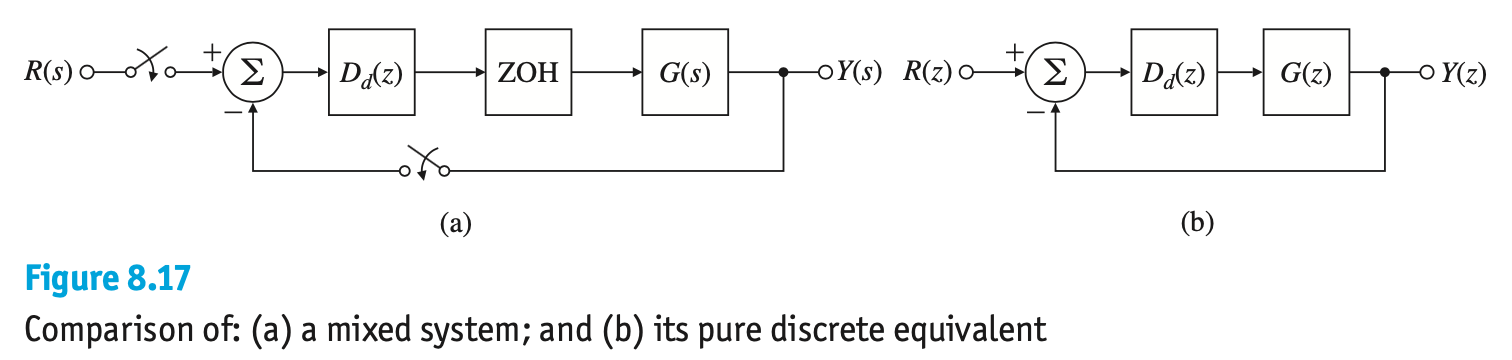
\includegraphics[width=12cm]{./FIG_Franklin/fig8-17.png}
	\end{figure}
	\item The closed-loop poles or the roots of the discrete characteristic equation
	\begin{align*}
		1+ D_d(z) G(z) = 0 
	\end{align*}
	\item The root-locus techniques used in continuous systems to find roots of a polynomial in $s$ apply equally well and without modification to the polynoimal in $z$.
	\item The interpretation of the results is that the stability boundary is now the unit circle instead of the imaginary axis. 
%
\end{itemize}
%

(Example 8.4)  When $G(s) = \frac{a}{s+a}$ and $D_d(z) = K$, draw the root locus with respect to $K$? 

(Answer) 
\begin{align*}
	G(z) &= (1-z^{-1}) \mathcal{Z} \left\{ \frac{a}{s(s+a)} \right\} = (1-z^{-1}) \mathcal{Z} \left\{ \frac{1}{s}  - \frac{1}{s+a} \right\} \\
	&= (1-z^{-1}) \left( \frac{1}{1-z^{-1}} - \frac{1}{1-e^{-aT}z^{-1}} \right)  \\
	&= \frac{(1-e^{-aT})z^{-1}}{1-e^{-aT}z^{-1}} \\
	&= \frac{(1-\alpha)z^{-1}}{1-\alpha z^{-1}} ~~~~~~~\mbox{where}~~ \alpha = e^{-aT}
\end{align*}
The discrete characteristic equation becomes
\begin{align*}
	1+ D_d(z) G(z) = 1 + K\frac{(1-\alpha)z^{-1}}{1-\alpha z^{-1}}= 0 
\end{align*}

\begin{figure}[h]
	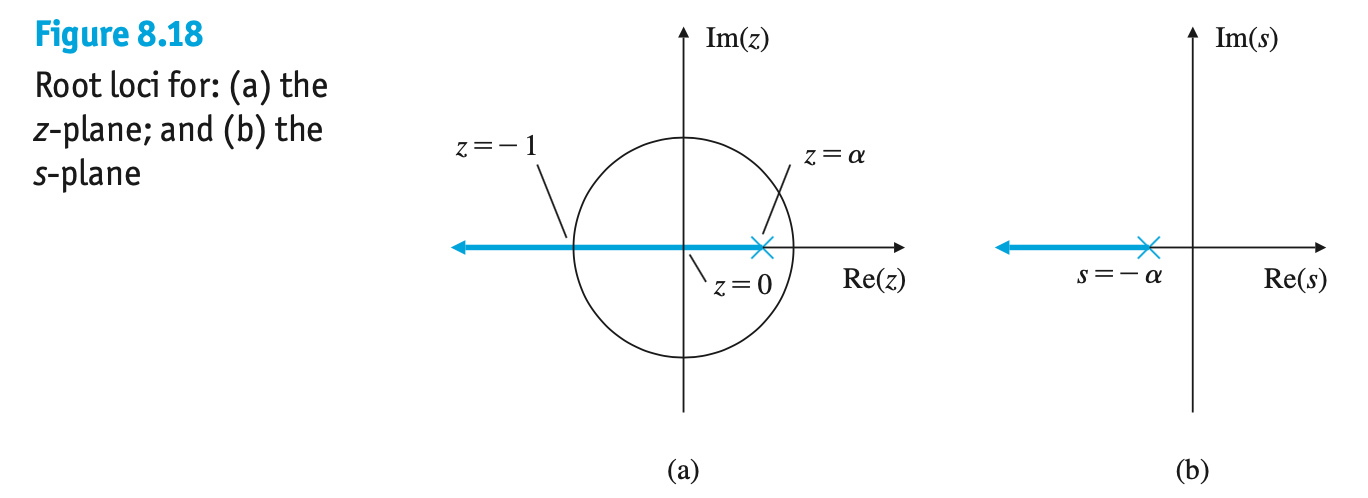
\includegraphics[width=12cm]{./FIG_Franklin/fig8-18.png}
\end{figure}

In the continuous case, the system remains stable for all values of $K$. 
In the discrete case, the system becomes oscillatory with decreasing damping ratio as $z$ goes from 0 to -1 and eventually becomes unstable. This instability is due to the lagging effect of the ZOH. 

%
\newpage
%
Feedback properties 
\begin{itemize}
	\item Proportional 
	\begin{align*}
		u(k) = Ke(k) ~~~~\leftrightarrow~~~~ D_d(z) = K 
	\end{align*}
	\item Derivative 
	\begin{align*}
		u(k) = K T_D [e(k) - e(k-1)] ~~~~~\leftrightarrow~~~~ D_d(z) = KT_D (1-z^{-1})
	\end{align*}
	\item Integral 
	\begin{align*}
		u(k) = u(k-1) + \frac{K}{T_I} e(k) ~~~~~\leftrightarrow~~~~ D_d(z) = \frac{K}{T_I} \left( \frac{1}{1-z^{-1}} \right) 
	\end{align*}
	\item Lead 
	\begin{align*}
		u(k) = \beta u(k-1) + K [e(k) - \alpha e(k-1)] ~~~~~\leftrightarrow~~~~ D_d(z) = K \frac{1- \alpha z^{-1}}{1-\beta z^{-1}} 
	\end{align*}
\end{itemize}
%
%
\newpage
%
%
\newpage
%
(Example 8.5)  Design a digital controller to have a closed-loop natural frequency $\omega_n = 0.3$ and a damping ratio $\zeta = 0.7$ using discrete design

(Answer) 
\begin{align*}
	G(s) = \frac{1}{s^2}   ~~~~~\rightarrow~~~~~~ G(z) = (1-z^{-1}) \mathcal{Z} \left\{ \frac{1}{s^3} \right\} = \frac{T^2}{2} \frac{z^{-1}(1+z^{-1})}{(1-z^{-1})^2}
\end{align*}
which, with $T=1$, becomes
\begin{align*}
	G(z) = \frac{1}{2} \frac{z^{-1}(1+z^{-1})}{(1-z^{-1})^2}
\end{align*}
Let us assume that the PD compensator is used
\begin{align*}
	D_d(z) = K (1- \alpha z^{-1})
\end{align*}
The desired pole locations of $\omega_n = 0.3$ and $\zeta = 0.7$ become $z=0.78 \pm 0.18j$ 
\begin{align*}
	1 + D_d(z) G(z) = 1 + K\frac{1}{2} \frac{z^{-1}(1+z^{-1})(1- \alpha z^{-1})}{(1-z^{-1})^2} =0 
\end{align*}
Now we have 
\begin{align*}
	\alpha = 0.85 ~~~~~~~~~~K = 0.374
\end{align*}
and 
\begin{align*}
	D_d(z) = 0.374 (1- 0.85 z^{-1})
\end{align*}
The difference equation becomes
\begin{align*}
	u(k) =  0.374 [e(k) - 0.85 e(k-1)] 
\end{align*}

(8장 숙제) 8장 연습문제에서 기말고사에 출제될 만한 문제 3개를 선택하여 풀어 제출하라? (마감 기말고사 전) 
% 
\newpage
   
    \newpage         


\end{document}
